%---------------------------------------------------------------
\chapter{Návrh}
%---------------------------------------------------------------

\begin{chapterabstract}
    V této kapitole se budu zabývat návrhem aplikace samotné. Nejprve popíšu případy užití a navrhnu architekturu aplikace, pak porovnám existující technologie pro tvorbu aplikací a vyberu tu nejvhodnější pro svou práci. V závěru pak navrhnu vhodný prototyp uživatelského rozhraní.
\end{chapterabstract}

\section{Případy užití}

Na základě provedené analýzy a jednotlivých funkčních požadavků jsem navrhl následující přípa\-dy užití:

\subsection{K1 Zobrazení textu aktuálně hrané písně}

\begin{enumerate}
    \item Věřící otevře aplikaci
    \item Aplikace zobrazí Přihlášení
    \item Věřící klikne na tlačítko \uv{Host}
    \item Aplikace zobrazí dialog Přihlášení -- kapela
    \item Věřící klikne na kapelu, jejíž aktuálně hranou píseň chce zobrazit
    \item Aplikace zobrazí Detail písně -- host
\end{enumerate}

\subsection{P1.1 Zobrazení seznamu všech písní}
\label{P1.1}

\begin{enumerate}
    \item Člen kapely otevře aplikaci
    \item Aplikace zobrazí Přihlášení
    \item Člen kapely stiskne tlačítko Přihlásit přes Apple
    \item Aplikace zobrazí dialog pro přihlášení přes Apple
    \begin{enumerate}
        \item Přihlášení bylo neúspěšné \emph{(uživatel přihlašování zamítl, nemá platný Apple účet)} -- aplikace zobrazí chybovou hlášku s možností zkusit přihlašování znovu
        \item Přihlášení bylo úspěšné -- aplikace zobrazí Seznam písní
    \end{enumerate}
\end{enumerate}

\subsection{P1.1.1 Filtrování seznamu všech písní}
\label{P1.1.1}

\begin{enumerate}
    \item Člen kapely postupuje podle scénáře \hyperref[P1.1]{P1.1}
    \item Člen kapely stiskne tlačítko Filtrovat
    \item Aplikace ukáže Seznam písní -- filtr
    \item Člen kapely vybere v zaškrtávacím seznamu jména zpěvníků, které chce zobrazit, případně stiskne tlačítko Zobrazit/skrýt vše
    \item Aplikace zobrazí v seznamu písní pouze písně z vyfiltrovaných zpěvníků
\end{enumerate}

\subsection{P1.1.2 Hledání v seznamu všech písní}
\label{P1.1.2}

\begin{enumerate}
    \item Člen kapely postupuje podle scénáře \hyperref[P1.1]{P1.1}
    \item Člen kapely zadá do vyhledávacího pole název, číslo, nebo text písně
    \item Aplikace zobrazí v seznamu písní pouze písně, které vyhovují zadanému číslu, názvu nebo textu
\end{enumerate}

\subsection{P1.2 Zobrazení detailu libovolné písně}

\begin{enumerate}
    \item Člen kapely postupuje dle scénáře \hyperref[P1.1]{P1.1}
    \item Člen kapely klikne na jméno písně, jejíž detail (text, akordy a poznámky) chce zobrazit
    \item Aplikace zobrazí Detail písně
\end{enumerate}

\subsection{P2 Zobrazení seznamu všech písní ve zpěvníku}
\label{P2}

\begin{enumerate}
    \item Člen kapely postupuje podle scénáře \hyperref[P1.1]{P1.1}
    \item Člen kapely stiskne šipku u jména zpěvníku, ze kterého chce zobrazit všechny písně
    \item Aplikace zobrazí Detail zpěvníku
\end{enumerate}

\begin{figure}
    \subsection{P3.2 + P6 Správa písní}
    \label{P3.2 + P6}
    \centering
    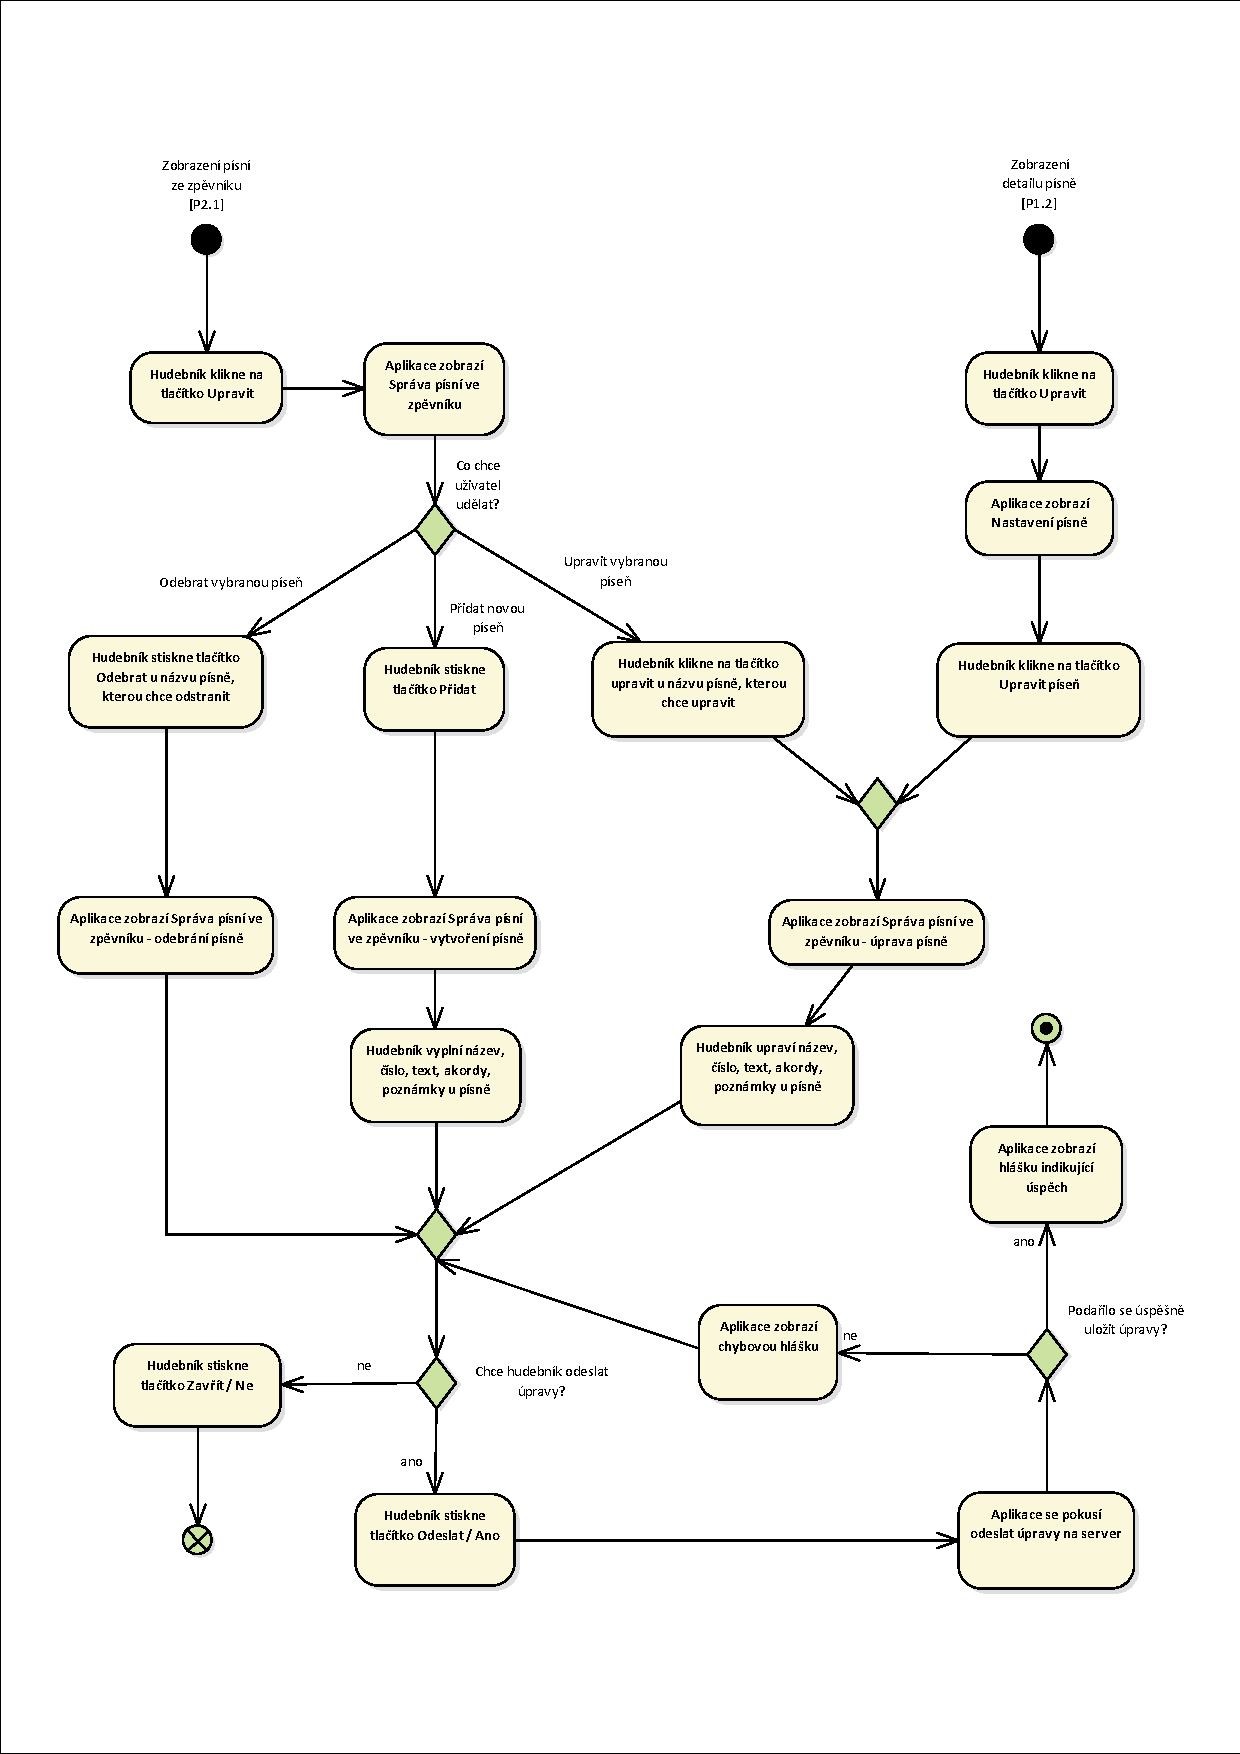
\includegraphics[width=\textwidth-8pt]{images/3-navrh/3-1-uc-sprava-pisni.pdf}
    \caption[Diagram případů užití Správa písní a Správa poznámek k písni]{Správa písní -- přidání nové písně, úprava a odebrání písně}
\end{figure}

\subsection{P3.1 Přidání nového zpěvníku}
\label{P3.1}

\begin{enumerate}
    \item Vedoucí postupuje dle scénáře \hyperref[P1.1]{P1.1}
    \item Vedoucí stiskne tlačítko Upravit
    \item Aplikace zobrazí Správa playlistů a zpěvníků
    \item Vedoucí stiskne tlačítko Přidat
    \item Aplikace zobrazí dialog Správa playlistu a zpěvníků - nový zpěvník
    \item Vedoucí vyplní informace o zpěvníku
    \item \begin{enumerate}
        \item Vedoucí chce přidat nový zpěvník -- stiskne Odeslat
        \item Vedoucí nechce přidat nový zpěvník -- stiskne Zavřít
    \end{enumerate}
    \item \begin{enumerate}
        \item Aplikace odešle žádost o vytvoření zpěvníku na server
        \item Aplikace zavře dialogové okno
    \end{enumerate}
    \item \begin{enumerate}
        \item \begin{enumerate}
            \item Vytvoření zpěvníku se podaří -- aplikace zobrazí dialog o úspěchu
	    \item Vytvoření zpěvníku je neúspěšné -- aplikace zobrazí chybový dialog
        \end{enumerate}
    \end{enumerate}
\end{enumerate}

\subsection{P3.3 Úprava zpěvníku}
\label{P3.3}

\begin{enumerate}
    \item Vedoucí postupuje dle bodu 1--3 scénáře \hyperref[P3.1]{P3.1}
    \item Vedoucí stiskne tlačítko Upravit u názvu zpěvníku, který chce upravit
    \item Aplikace zobrazí dialog Správa playlistu a zpěvníků - úprava zpěvníku
    \item Vedoucí vyplní nové informace o zpěvníku
    \item \begin{enumerate}
        \item Vedoucí chce upravit zpěvník -- stiskne Odeslat
        \item Vedoucí nechce upravit zpěvník -- stiskne Zavřít
    \end{enumerate}
    \item \begin{enumerate}
        \item Aplikace odešle žádost o úpravu zpěvníku na server
        \item Aplikace zavře dialogové okno
    \end{enumerate}
    \item \begin{enumerate}
        \item \begin{enumerate}
            \item Úprava zpěvníku se podaří -- aplikace zobrazí dialog o úspěchu
	    \item Úprava zpěvníku je neúspěšná -- aplikace zobrazí chybový dialog
        \end{enumerate}
    \end{enumerate}
\end{enumerate}

\subsection{P3.4 Odebrání zpěvníku}
\label{P3.4}

\begin{enumerate}
    \item Vedoucí postupuje podle bodu 1--3 scénáře \hyperref[P3.1]{P3.1}
    \item Vedoucí stiskne tlačítko Odebrat u názvu zpěvníku, který chce odebrat
    \item Aplikace zobrazí dialog Správa playlistu a zpěvníků - odebrání zpěvníku
    \item \begin{enumerate}
        \item Vedoucí chce odebrat zpěvník -- stiskne Ano
	\item Vedoucí nechce odebrat zpěvník -- stiskne Ne
    \end{enumerate}
    \item \begin{enumerate}
        \item Aplikace odešle žádost o odebrání zpěvníku na server
	\item Aplikace zavře dialogové okno
    \end{enumerate}
    \item \begin{enumerate}
        \item \begin{enumerate}
            \item Odebrání zpěvníku se podaří -- aplikace zobrazí dialog o úspěchu
	    \item Odebrání zpěvníku je neúspěšné -- aplikace zobrazí chybový dialog
        \end{enumerate}
    \end{enumerate}
\end{enumerate}

\subsection{P4.1 Přidání libovolné písně do playlistu}
\label{P4.1}

Přidat píseň do playlistu lze dvěma způsoby -- scénář 1 je optimalizován pro přidání jedné písně, pro případ přidávání více písní je optimalizován scénář 2.

\subsubsection{P4.1.1 Přidání jedné písně do playlistu}
\label{P4.1.1}

\begin{enumerate}
    \item Člen kapely postupuje dle scénáře \hyperref[P1.1]{P1.1}
    \item Člen kapely dlouze podrží prst na názvu písně, kterou chce exportovat k tisku
    \item Aplikace zobrazí Seznam písní -- kontextová nabídka
    \item Člen kapely vybere z kontextové nabídky možnost Přidat do playlistu
    \item Aplikace přidá danou píseň na konec playlistu
\end{enumerate}

\subsubsection{P4.1.2 Přidání více písní do playlistu}
\label{P4.1.2}

\begin{enumerate}
    \item Člen kapely postupuje dle scénáře \hyperref[P1.1]{P1.1}
    \item Člen kapely stiskne tlačítko Upravit
    \item Aplikace zobrazí Správa playlistu a zpěvníků
    \item Člen kapely stiskne tlačítko Přidat u názvu písní, které chce přidat do playlistu
    \item Aplikace přidá dané píseň na konec playlistu
\end{enumerate}

\subsection{P4.2 Úprava pořadí písní v playlistu}
\label{P4.2}

\begin{enumerate}
    \item Člen kapely postupuje dle scénáře \hyperref[P4.1.1]{P4.1.1}
    \item Člen kapely potáhne píseň z playlistu na požadovanou pozici v rámci playlistu
    \item Aplikace provede požadovanou změnu pořadí písní v playlistu
\end{enumerate}

\subsection{P4.3 Odebrání libovolné písně z playlistu}
\label{P4.3}

Odebrání písně z playlistu je stejně jako u přidávání písní do playlistu možné dvěma způsoby, kdy scénář 1 je optimalizován pro odebírání jedné písně a scénář 2 pro odebírání více písní.

\subsubsection{P4.3.1 Odebrání jedné písně z playlistu}
\label{P4.3.1}

\begin{enumerate}
    \item Člen kapely postupuje dle scénáře \hyperref[P1.1]{P1.1}
    \item Člen kapely potáhne doleva název písně, kterou chce odebrat z playlistu
    \item Aplikace odebere píseň z playlistu
\end{enumerate}

\subsubsection{P4.3.2 Odebrání více písní z playlistu}
\label{P4.3.2}

\begin{enumerate}
    \item Člen kapely postupuje dle bodu 1--3 scénáře \hyperref[P4.1.2]{P4.1.2}
    \item Člen kapely stiskne Odebrat u názvu písní, které chce odebrat z playlistu
    \item Aplikace odebere požadované písně z playlistu
\end{enumerate}

\subsection{P5.1 Zobrazení detailu kapely}
\label{P5.1}

\begin{enumerate}
    \item Člen kapely postupuje podle scénáře \hyperref[P1.1]{P1.1}
    \item Člen kapely klikne na Nastavení
    \item Aplikace zobrazí Nastavení
    \item Člen kapely vybere kapelu, jejíž detail chce zobrazit
    \item Aplikace zobrazí Nastavení -- detail kapely
\end{enumerate}

\begin{figure}
    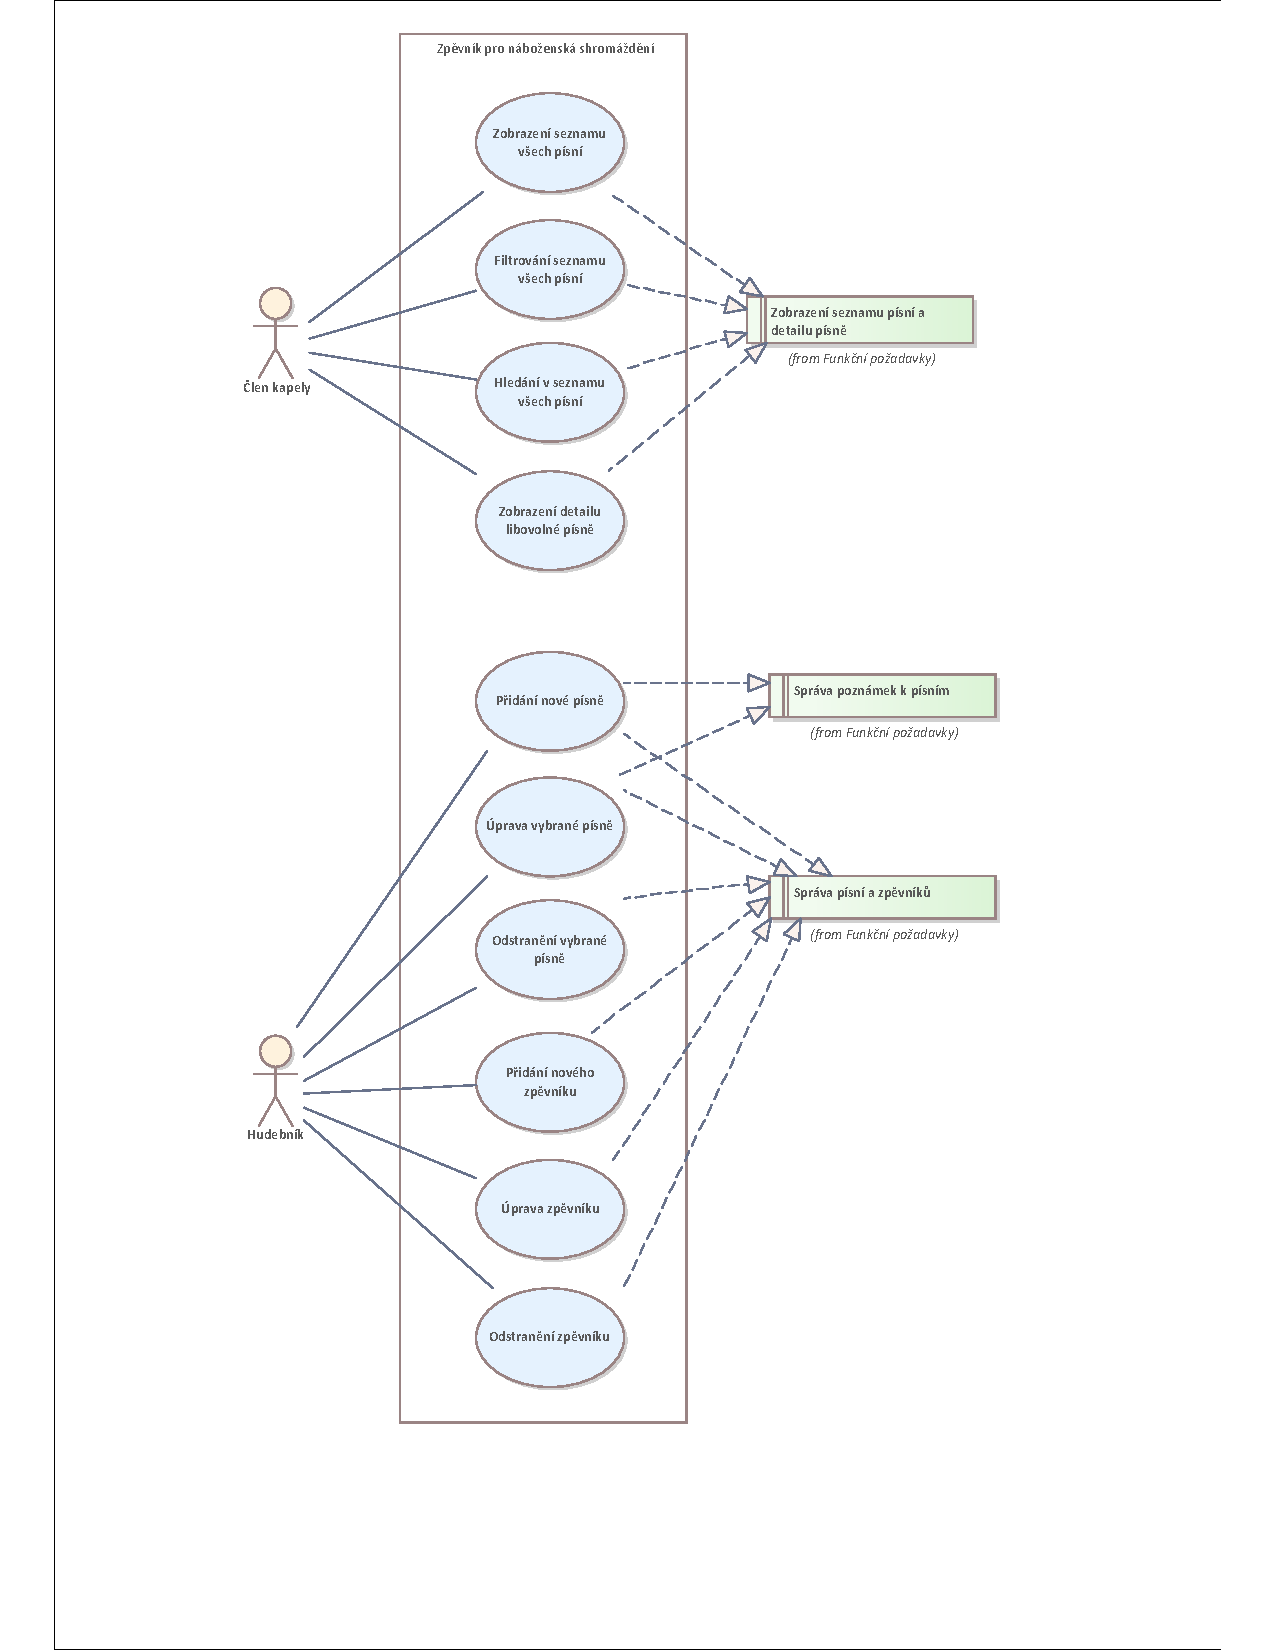
\includegraphics[width=\textwidth]{images/3-navrh/3-2-uc-model-1.pdf}
    \caption{Model případů užití -- člen kapely a hudebník}
\end{figure}

\begin{figure}
    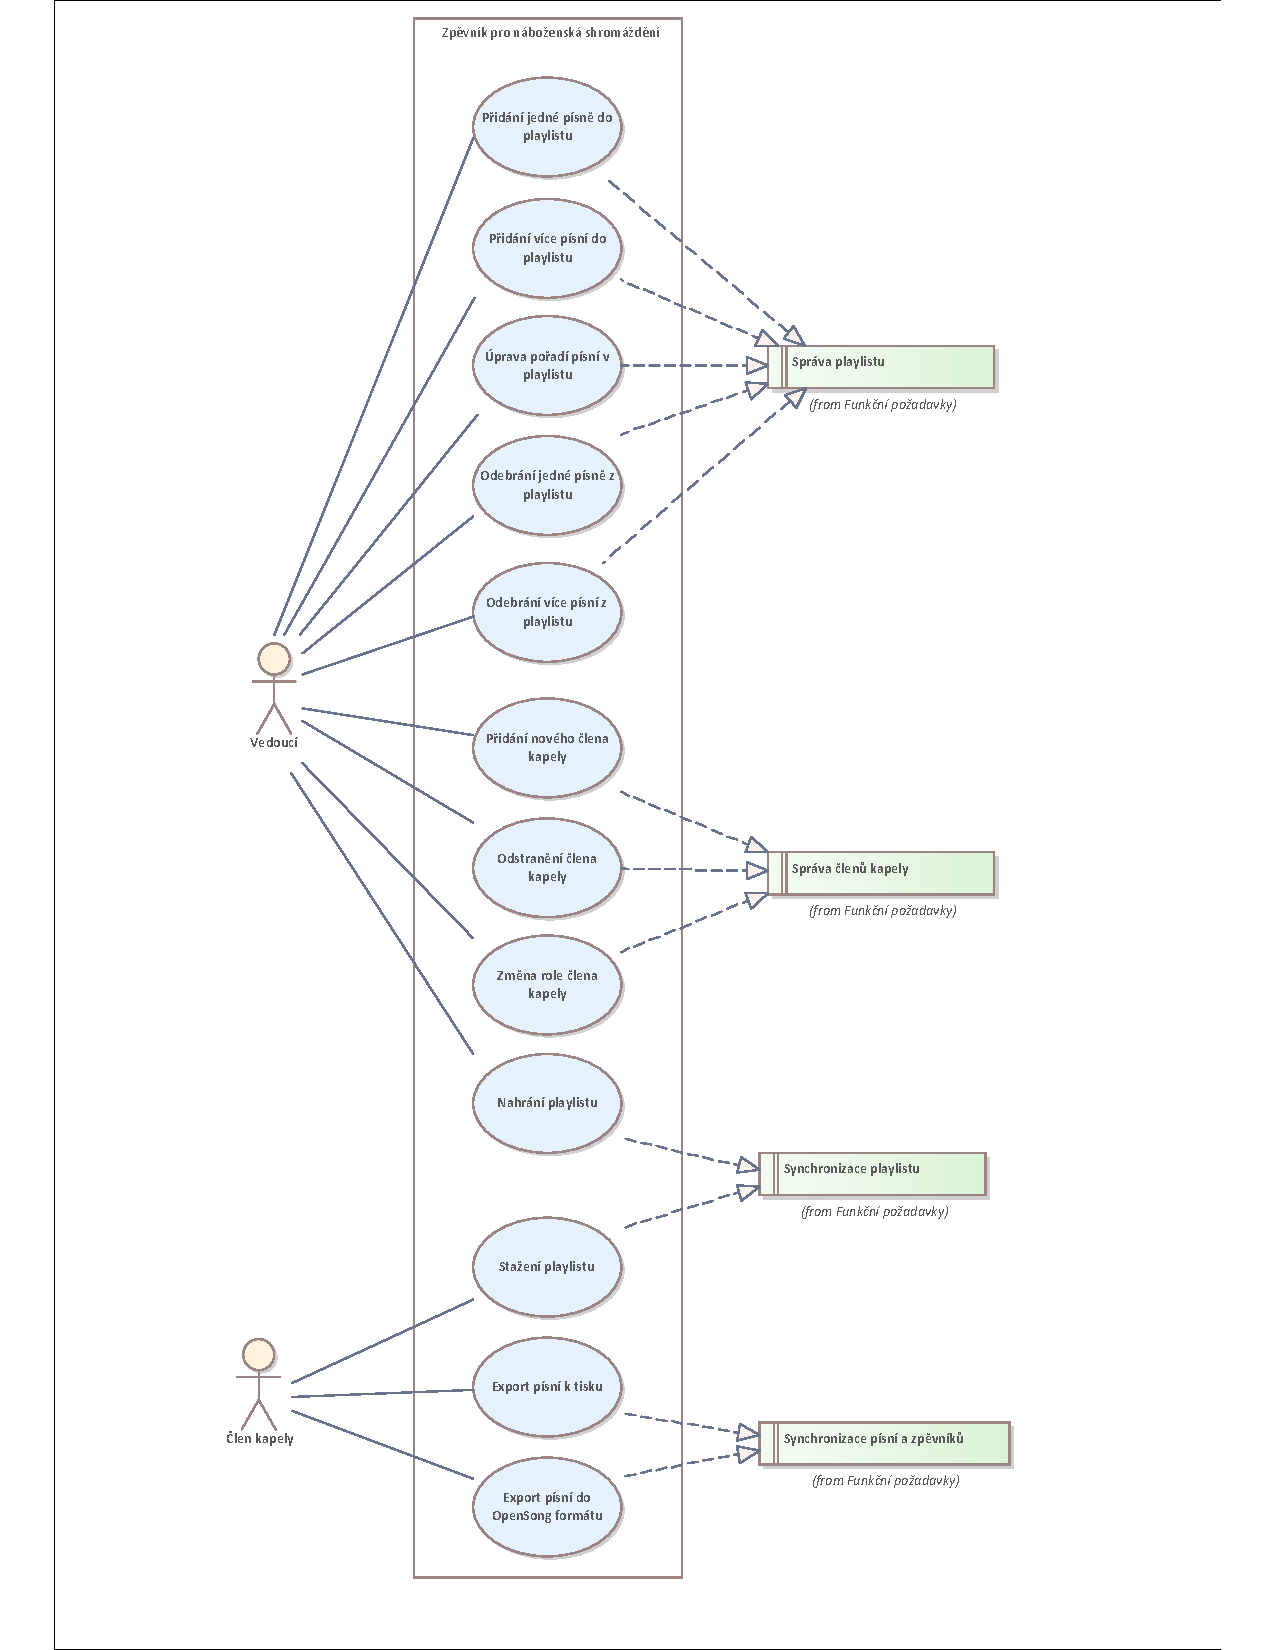
\includegraphics[width=\textwidth]{images/3-navrh/3-3-uc-model-2.pdf}
    \caption{Model případů užití -- vedoucí a člen kapely}
\end{figure}

\subsection{P5.2 Přidání nového člena kapely}
\label{P5.2}

\begin{enumerate}
    \item Vedoucí postupuje podle scénáře \hyperref[P5.1]{P5.1}
    \item Vedoucí klikne na tlačítko Upravit
    \item Aplikace zobrazí Nastavení -- správa kapely
    \item Vedoucí klikne na tlačítko Přidat
    \item Aplikace zobrazí dialog Nastavení -- nový člen kapely
    \item Vedoucí vyplní údaje nového člena
    \item \begin{enumerate}
        \item Vedoucí nového člena chce přidat -- stiskne Odeslat
        \item Vedoucí nového člena nechce přidat -- stiskne Zavřít
    \end{enumerate}
    \item \begin{enumerate}
        \item Aplikace odešle žádost o přidání nového člena
        \item Aplikace zavře dialogové okno
    \end{enumerate}
    \item \begin{enumerate}
        \item \begin{enumerate}
            \item Přidání člena se podaří -- aplikace zobrazí dialog s informací o úspěchu
            \item Přidání člena je neúspěšné -- aplikace zobrazí chybový dialog
        \end{enumerate}
    \end{enumerate}
\end{enumerate}

\subsection{P5.3 Odebrání člena kapely}
\label{P5.3}

\begin{enumerate}
    \item Vedoucí postupuje podle bodu 1--3 scénáře \hyperref[P5.2]{P5.2}
    \item Vedoucí klikne na Odebrat u člena kapely, kterého chce odebrat
    \item Aplikace zobrazí dialog Nastavení - odebrání člena kapely
    \item \begin{enumerate}
        \item Vedoucí člena chce odebrat -- stiskne Ano
        \item Vedoucí člena nechce odebrat -- stiskne Ne
    \end{enumerate}
    \item \begin{enumerate}
        \item Aplikace odešle žádost o odebrání člena
        \item Aplikace zavře dialogové okno
    \end{enumerate}
    \item \begin{enumerate}
        \item \begin{enumerate}
            \item Odebrání člena se podaří -- aplikace zobrazí dialog s informací o úspěchu
            \item Odebrání člena je neúspěšné -- aplikace zobrazí chybový dialog
        \end{enumerate}
    \end{enumerate}
\end{enumerate}

\subsection{P5.4 Změna role člena kapely}
\label{P5.4}

\begin{enumerate}
    \item Vedoucí postupuje podle bodu 1--3 scénáře \hyperref[P5.2]{P5.2}
    \item Vedoucí klikne na Zvýšit oprávnění nebo Snížit oprávnění u člena kapely, kterému chce změnit roli
    \item Aplikace zobrazí dialog Nastavení - změna role člena kapely
    \item \begin{enumerate}
        \item Vedoucí členovi chce změnit roli -- stiskne Ano
        \item Vedoucí členovi nechce změnit roli -- stiskne Ne
    \end{enumerate}
    \item \begin{enumerate}
        \item Aplikace odešle žádost o změnu role
        \item Aplikace zavře dialogové okno
    \end{enumerate}
    \item \begin{enumerate}
        \item \begin{enumerate}
            \item Změna role se podaří -- aplikace zobrazí dialog s informací o úspěchu
            \item Změna role je neúspěšná -- aplikace zobrazí chybový dialog
        \end{enumerate}
    \end{enumerate}
\end{enumerate}

\subsection{P7.1 Export písní k tisku}
\label{P7.1}

\begin{enumerate}
    \item Člen kapely postupuje dle scénáře \hyperref[P1.1]{P1.1}
    \item Člen kapely dlouze podrží prst na názvu písně, kterou chce exportovat k tisku
    \item Aplikace zobrazí Seznam písní -- kontextová nabídka
    \item Člen kapely vybere z kontextové nabídky možnost Exportovat k tisku
    \item Aplikace otevře prohlížeč se stránkou s vygenerovaným textem k tisku
\end{enumerate}

\subsection{P7.2 Export písní do OpenSong formátu}
\label{P7.2}

\begin{enumerate}
    \item Člen kapely postupuje podle bodu 1--2 scénáře \hyperref[P7.1]{P7.1}
    \item Člen kapely vybere z kontextové nabídky možnost Exportovat do OpenSong
    \item Aplikace otevře prohlížeč se stránkou s vygenerovanou písní v OpenSong formátu
\end{enumerate}

\subsection{P8.1 Nahrání playlistu}
\label{P8.1}

\begin{enumerate}
    \item Vedoucí postupuje podle scénáře \hyperref[P1.1]{P1.1}
    \item Vedoucí stiskne tlačítko Nahrát u nadpisu Playlist
    \item Aplikace zobrazí Správa playlistu a zpěvníků - výběr kapely
    \item Vedoucí vybere kapelu, do které chce nahrát playlist
    \item Aplikace se pokusí odeslat playlist na server
    \item \begin{enumerate}
        \item Playlist se nepodařilo uložit -- aplikace zobrazí chybovou hlášku
        \item Playlist se podaří uložit -- aplikace zobrazí hlášku o úspěšném uložení
    \end{enumerate}
\end{enumerate}

\subsection{P8.2 Stažení playlistu}
\label{P8.2}

\begin{enumerate}
    \item Člen kapely postupuje podle scénáře \hyperref[P1.1]{P1.1}
    \item Člen kapely stiskne tlačítko Stáhnout u nadpisu Playlist
    \item Aplikace zobrazí Správa playlistu a zpěvníků - výběr kapely
    \item Člen kapely vybere kapelu, ze které chce stáhnout playlist
    \item Aplikace se pokusí stáhnout playlist ze serveru
    \item \begin{enumerate}
        \item Playlist se nepodařilo stáhnout -- aplikace zobrazí chybovou hlášku
        \item Playlist se podaří stáhnout -- aplikace zobrazí hlášku o úspěšném uložení
    \end{enumerate}
\end{enumerate}

\section{Architektura aplikace}

Jelikož většina členů hudebního doprovodu aktivně používá zařízení s operačním systémem iOS nebo macOS, vznikl na aplikaci nefunkční požadavek na podporu těchto platforem. Vzhledem k možnému budoucímu rozšíření na další mobilní platformy nebo na web vznikl také nefunkční požadavek na API rozhraní. Na základě těchto dvou nefunkčních požadavků jsem se rozhodl aplikaci koncipovat jako multiplatformní klientskou aplikaci pro operační systém iOS a macOS a podpůrný server poskytující API rozhraní. V aplikaci budu také ukládat písně, zpěvníky a uživatele, budu tedy potřebovat databázi, se kterou bude server komunikovat.

\begin{figure}
    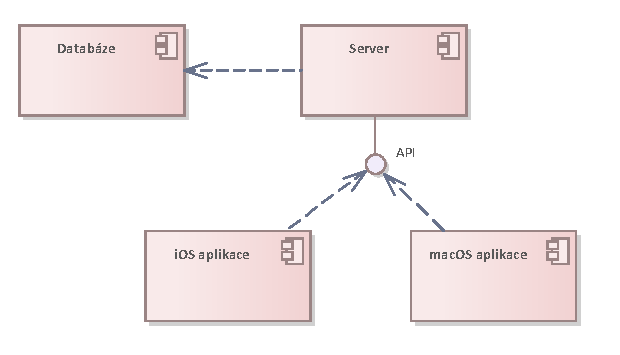
\includegraphics[width=\textwidth]{images/3-navrh/3-4-diagram-komponent.pdf}
    \caption[Diagram komponent aplikace]{Diagram komponent -- Databáze, server, API, iOS a macOS aplikace}
\end{figure}

\section{Databáze}

Existuje více způsobů, kterými může aplikace ukládat data. Jednotlivé způsoby se liší v rychlosti a efektivitě ukládání dat, v typu ukládaných dat a na základě dotazů, které budou nad daty prováděny. Tyto způsoby porovnám, a zvolím nejvhodnější pro svou aplikaci.

\subsection{Operační paměť}

Data aplikace můžou být uložena přímo v operační paměti. Toto řešení je vhodné pro dočasná data, které nemusí přežít restart aplikace. Výhodou operační paměti je také rychlost získání takto uložených dat. Pro ukládání zpěvníků, písní a dat uživatelů operační paměť nebude vhodné řešení, jelikož potřebuji, aby tato data přežila restart aplikace.

\subsection{Soubory}

Jednou z možností je ukládat data do souboru. Data do souboru můžeme ukládat v různých nestrukturovaných či strukturovaných formátech.

\begin{figure}[H]
    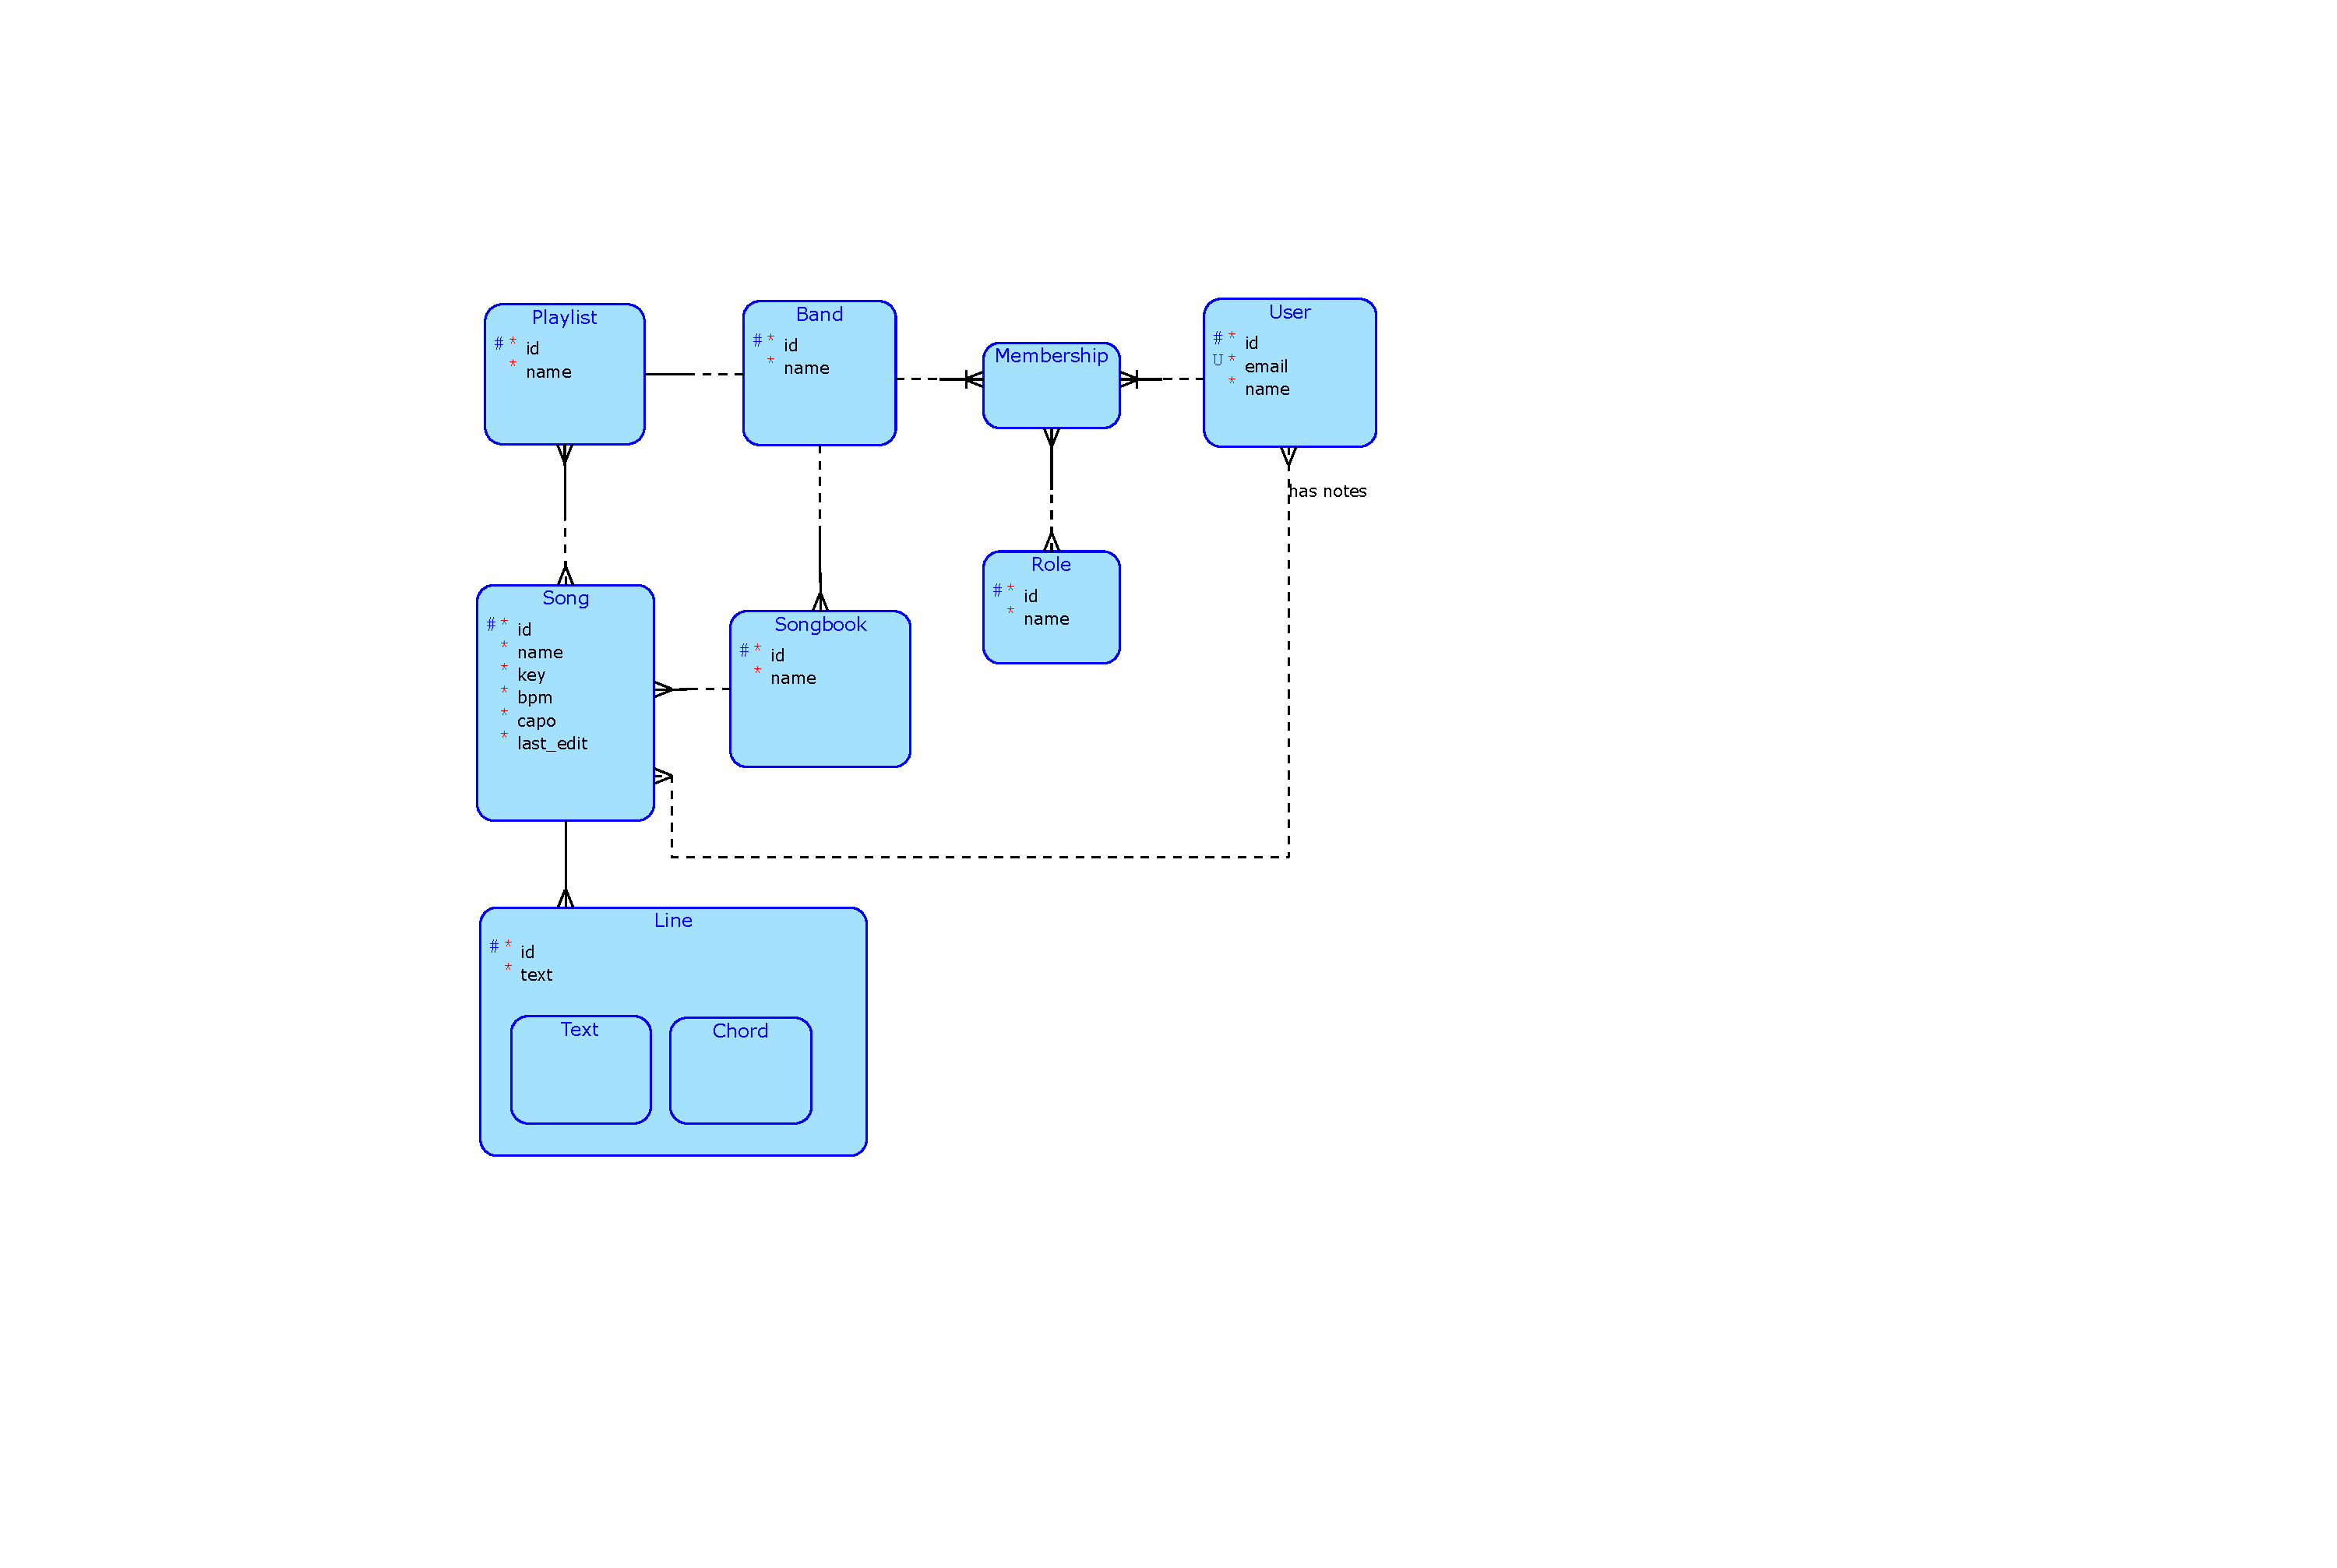
\includegraphics[width=\textwidth]{images/3-navrh/3-5-konceptualni-model.pdf}
    \caption{Konceptuální model aplikace}
\end{figure}

Nevýhodou tohoto způsobu ukládání dat je nutnost řešení problému souběžného zápisu, v~případě většího množství ukládaných dat je pak vyhledávání v datech pomalé a neefektivní. Tento způsob je vhodný pro ukládání binárních dat, jako jsou obrázky a videa. Pro data aplikace toto řešení taktéž nebude vhodné, jelikož aplikaci může používat více uživatelů najednou, a v~takovém případě by u práce se soubory mohl nastat problém při souběžném zápisu.

\subsection{Relační databáze}

Relační databáze jsou v dnešním době jedním z nejpoužívanějších řešení ukládání dat. Řeší problém souběžného zápisu a umožňují strukturované uložení dat, nad kterými lze vybudovat indexy pro rychlejší vyhledávání. \cite{what-is-rdbms}

Nevýhodou relačních databází je problematické ukládání velkého množství dat nebo binárních souborů, jako jsou obrázky a videa. Práce s daty v relační databázi je rychlá a jednoduchá díky dotazovacímu jazyku SQL. Relační databáze splňuje všechny požadavky pro uložení dat aplikace.

\subsection{NoSQL databáze}

Tradiční relační databáze byly navrženy ještě před vznikem internetu a mobilních aplikací tak, aby běžely na jediném, vertikálně škálovatelném serveru -- jedinou možností zvětšení výkonu byla koupě lepšího procesoru a paměti. NoSQL databáze umožňují horizontální škálování -- výkon je navýšen koupením většího počtu méně výkonných serverů. Oproti tradičním relačním databázím pak mají NoSQL databáze typicky volnější datové schéma a jelikož jsou informace uloženy na~více serverech, dochází k jejich duplicitám. \cite{why-nosql} O datech aplikace vím, že písní budou maximálně tisíce a uživatelů budou desítky -- nebudu tedy potřebovat databázi škálovat. Při práci s daty v~aplikaci navíc potřebuji, aby byla data aktuální a přesná.

\subsection{Zvolená databáze}

Po porovnání existujících technologií ukládání dat jsem dospěl k závěru, že pro mou aplikaci bude nejvhodnější data ukládat do relační databáze. Mezi nejčastěji používané relační databáze patří MySQL \cite{mysql}, MariaDB \cite{mariadb}, PostgreSQL \cite{postgresql}, Oracle Database \cite{oracle} a Microsoft SQL Database \cite{mssql}. Poslední dvě jmenovaná řešení, Oracle Database a Microsoft SQL Database jsou komerční řešení, ostatní opensource. Komerční řešení by byla pro účely mé bakalářské práce zbytečně příliš komplexní a drahá, rozhodl jsem se proto pro opensource řešení. Mezi MySQL, MariaDB a PostgreSQL jsem se rozhodl pro MySQL, jelikož již vlastním server s MySQL databází, který pro účely bakalářské práce můžu využít bez nutnosti nastavování nového serveru a také proto, že mám s tímto řešením největší zkušenosti.

\section{Architektura API}

API, z anglického Application Programming Interface, je mostem mezi více oddělenými aplikacemi. Architektura API je určena významem a podobou zpráv, které je API schopno zpracovávat. V průběhu let byly vytvořeny různé styly API architektury, kde každý z nich má vlastní schéma výměny dat. Diskuze, která architektura je nejlepší, tak nemá konec. \cite{altexsoft}

\subsection{SOAP}

SOAP, z anglického Simple Object Access Protocol, zpřístupňuje data v XML (eXtended Markup Language) formátu a je silně standardizovaný. Byl vytvořen Microsoftem v roce 1999. SOAP zpráva se skládá z počáteční a koncové značky, těla s požadavkem nebo odpovědí, nepovinné hlavičky a informací o případných chybách. SOAP API je napsáno v WSDL (Web Service Description Language) popisem endpointů (= adresa, se kterou lze komunikovat) a popisem všech akcí, které lze provést. Výhodou SOAPu je jeho nezávislost na platformě a programovacím jazyce, vestavěné zpracování chyb a různá bezpečnostní rozšíření -- proto se často používá pro přenos dat u bank a korporátů. Velkou nevýhodou je nutnost použití XML, která způsobuje, že přenášené datové zprávy jsou velké. \cite{altexsoft}

Jedním z problémů použití architektury SOAP pro mou aplikaci je velikost přenášených dat, kdy u mobilních aplikací platí, že čím méně dat aplikace potřebuje, tím lépe. Využití SOAP by tak mohlo způsobit vysokou datovou spotřebu aplikace a zhoršení uživatelského zážitku. Z~hlediska programování by pak byl návrh SOAP API časově zbytečně velmi náročný, což není nutné vzhledem k tomu, že na systém není požadavek na vysokou bezpečnost.

\subsection{REST}

REST, z anglického REpresentational State Transfer, je samopopisná architektura API pocháze\-jící z roku 2000. REST podporuje různé formáty, nejčastěji XML a JSON. REST není silně standardizovaný, musí ale splňovat určité požadavky, mezi které patří architektura klient-server, umožňující nezávislý vývoj jak klienta, tak serveru a bezestavovost, kdy veškerá data potřebná k zpracování požadavku jsou obsažena v požadavku samotném, sever tedy nemusí ukládat dodatečná data.

Komunikace s REST API probíhá pomocí volání endpointů, které reprezentují jednotlivé zdroje. Operace s těmito zdroji jsou pak prováděny pomocí metod protokolu HTTP. Velkou výhodou RESTu je jeho samopopisnost, kdy při použití HATEOAS (Hypertext As The Engine of Application State) je u každého požadavku uvedena sada metadat odkazujících na informace, jak API používat. Nevýhodou použití HATEOAS je ale hodně metadat, která způsobují, že zprávy jsou velké. \cite{altexsoft}

Datový formát JSON je nativně podporován většinou programovacích jazyků pro tvorbu mobilních aplikací. Při vypnutí HATEOAS navíc aplikace nebude mít vysokou datovou spotřebu. Návrh a naprogramování REST API je pak časově méně náročné než například návrh a naprogramování SOAP API.

\subsection{GraphQL}

GraphQL \cite{graphql} je architektura umožňující provedení přesného požadavku. Použití GraphQL je vhodné, pokud data obsahují hodně komplexních entit, které se k sobě vztahují. Návrh GraphQL spočívá ve vytvoření schématu všech dotazů, které lze provést a všech datových typů, které můžou být vráceny v odpovědi. To zajišťuje, že server dokáže na požadavek vždy odpovědět a data jsou vrácena přesně v podobě, která je požadována. Nevýhodou je ale složitost zachování požadavků a také množství práce před začátkem vývoje. \cite{altexsoft}

Programovací jazyky pro tvorbu mobilních aplikací GraphQL nativně nepodporují, pro jeho použití je potřeba využít externí knihovnu, jakou je například Apollo GraphQL \cite{apollo-graphql}. Aplikace navíc nebude potřebovat provádět komplexní dotazy a použití GraphQL by bylo časově náročnější než použití REST.

\subsection{Zvolená architektura}

Na základě analýzy existujících řešení pro architekturu API jsem se rozhodl si vybrat architekturu REST, která nejlépe odpovídá požadavkům -- nedochází zde k velkému objemu přenášených zpráv, návrh je v porovnání s ostatními architekturami nejméně náročný a architektura REST je nativně podporována většinou programovacích jazyků pro psaní mobilních aplikací.

\section{Návrh REST API}

Z konceptuálního modelu vyplývá, že jednotlivé zdroje budou uživatel (/user), kapela (/band), zpěvník (/songbook) a píseň (/song).

\subsection{Zdroj /user}

Na uživateli bude přístupný zdroj POST /user/login, který umožní přihlášení uživatele na základě e-mailu a hesla nebo přihlašovacího klíče. Pokud se do systému pokusí přihlásit neexistující uživatel, bude mu vytvořena nová kapela, ve které bude nastaven jako vedoucí.

\subsection{Zdroj /band}

Systém umožní získat seznam všech kapel (GET /), včetně jejich členů a rolí. Kapely následně půjde také vytvářet (POST /), upravovat (PATCH /id) a také mazat (DELETE /id).

Nad kapelou bude možné přidávat členy (POST /id/members). API také umožní jednotlivým členům (/id/members/memberId) měnit role (PATCH) nebo členy z kapely odebrat (DELETE).

Každá kapela bude mít svůj playlist (/id/playlist), který půjde získat (GET) a také nahradit (PUT).

\subsection{Zdroje /songbook a /song}

Systém umožní získat seznam všech zpěvníků, včetně písní v nich obsažených (GET /songbook). Zpěvníky umožní také vytvářet (POST /songbook), upravovat (PATCH /songbook/id) a mazat (DELETE /songbook/id).

Systém umožní také přidávání písní (POST /song), jejich úpravu (PATCH /song/id), odebrá\-ní (DELETE /song/id) a nastavení poznámek k písni (PUT /songbook/songBookId/songs/song\allowbreak{}Id/notes).

\section{Architektura serveru}

Pro server jsem zvolil třívrstvou architekturu MVC (Model View Controller). Na datové vrstvě se nachází balíčky Entity a Repository, které mají na starost získávání dat z databáze. V business vrstvě se nachází balíčky DTO a Service, které zpracovávají logiku aplikace. V prezentační vrstvě se pak nachází balíček Controller, který poskytuje navrhnuté API rozhraní.

\section{Technologie pro server}

REST API, které jsem navrhnul, poběží na serveru s pomocí jedné z možných technologií. Výběr technologie závisí většinou na zvoleném programovacím jazyce. U každého z programovacích jazyků tak porovnám dostupné technologie podle následujících kritérií: cena, vhodnost, náročnost a moje zkušenost. Podle těchto kritérií pak určím nejvhodnější technologii, s pomocí které server naimplementuji.

\subsection{PHP}
\label{symfony}

PHP \cite{php} je dynamicky typovaný programovací jazyk určen primárně pro vývoj webových aplikací. Existují v něm různé frameworky, s jejichž pomocí lze navrhnout REST API, ať už se jedná o Slim \cite{slim}, Nette \cite{nette} nebo Symfony \cite{symfony}. PHP je možné spustit na většině webových hostingů za cenu (včetně domény) do tisíce korun ročně v konfiguraci s dostatečným výkonem. Nasazení na~takový webový hosting je otázkou několika minut, kdy stačí webovou aplikaci na~hosting pouze nahrát. S programovacím jazykem PHP mám dlouholeté zkušenosti, o konkrétních technologiích mám pouze základní povědomí.

\subsection{C\#}
\label{asp-net}

C\# \cite{csharp} je staticky typovaný programovací jazyk. Je v něm napsán framework ASP.NET \cite{dotnet}, který umožňuje mimo klasické webové aplikace také návrh REST API. Jedná se o řešení zaměřené na firmy, které je úzce integrované s operačním systémem Windows. Nasazení je možné na~virtu\-ální stroj, který se včetně domény dá pořídit také do tisíce korun ročně. Nasazení je ale časově náročnější, jelikož je zde nutnost nastavení vývojového prostředí a balíčků na virtuálním stroji. S programovacím jazykem C\# ani frameworkem ASP.NET nemám žádné zkušenosti.

\subsection{Java a Kotlin}

Java \cite{java} je staticky typovaný programovací jazyk, ve kterém je napsán framework Spring Web \cite{spring-web} umožňující tvorbu webových aplikací. Nasazení je taktéž možné na virtuální stroj, platí zde tedy z hlediska ceny a obtížnosti nasazení totéž, co u \hyperref[asp-net]{ASP.NET}. S frameworkem Spring Web mám bohaté zkušenosti z bakalářského studia, kdy jsem jej využil pro tvorbu semestrálních prací v předmětech Technologie Java a Softwarové inženýrství.

Kotlin \cite{kotlin} je nový programovací jazyk od firmy Jetbrains, který běží na Java Virtual Machine. Je v něm napsán nový webový framework Ktor \cite{ktor}, který ale prozatím není ještě doladěný a nemám s ním mnoho zkušeností. Pro Ktor také není dostupná tak rozsáhlá podpora jako u~technologií typu \hyperref[symfony]{Symfony} nebo Spring Web, které jsou hojně využívané.

Kotlin běží v Java Virtual Machine, což jej činí plně kompatibilním s veškerými knihovnami napsanými v programovacím jazyce Java, a to včetně frameworku Spring Web. Kotlin je mnohem modernější jazyk, ve kterém se díky bohatým rozšířením dá napsat kód mnohem snadněji a srozumitelněji než v Javě. Proto jsem v předmětu Programování v Kotlinu naprogramoval nadstavbu nad Kotlin verzí frameworku Spring Web, která umožňuje velmi rychlé a efektivní vytvoření REST API.

\subsection{Zvolená technologie}

Na základě provedené analýzy jsem dospěl k závěru, že nejvhodnější technologií bude framework Spring Web s použitím mé nadstavby v programovacím jazyce Kotlin, a to na základě přívětivé ceny, dlouholetých zkušeností s tímto frameworkem a programovacím jazykem a rozsáhlého množství dostupných knihoven v jazycích Kotlin i Java.

\section{Architektura mobilní aplikace}

Pro vývoj aplikací pro iOS a macOS se dnes využívá už pouze programovací jazyk Swift \cite{swift}, který nahradil původní programovací jazyk Objective C. Pro tvorbu aplikace lze využít dvě architektury -- Model View Controller (MVC) a Model View ViewModel (MVVM). \cite{mvc-mvvm}

\subsection{MVC}

Architektura MVC (Model View Controller) se skládá ze tří balíčků -- Model, což jsou pouze datové struktury bez jakékoliv logiky, View obsahující definici a popis vzhledu aplikace a Controller, který řeší veškerou logiku a komunikuje s jednotlivými View. \cite{mvc-mvvm} Nevýhodou této architektury je právě fakt, že Controller obsahuje jak business, tak prezentační logiku, a dochází tedy k velkým a nepřehledným Controllerům.

\subsection{MVVM}

Architektura MVVM (Model View ViewModel) se skládá ze tří balíčků -- Model, tedy opět datové struktury bez logiky, View, které obsahují definici a popis vzhledu a chování aplikace a ViewModel, který drží data, řeší business logiku a se kterým komunikují View. \cite{mvc-mvvm} Nevýhodou této architektury je to, že pokud nejsou jednotlivá View dostatečně rozdělena na menší View, nastává podobný problém jako u MVC -- dochází k velkým a nepřehledným View.

\subsection{Zvolená architektura}

Na základě analýzy architektur MVC a MVVM jsem se rozhodl použít architekturu MVVM, která je modernější, používanější a přehlednější. Při návrhu si pak budu dávat pozor na to, abych jednotlivá View dostatečně rozdělil a nedošlo tedy k jejich nepřehlednosti.

\section{Technologie pro mobilní aplikaci}

Existují dva zásadní směry, kterými se dá jít při vývoji mobilní aplikace: hybridní aplikace (tedy taková, která podporuje více platforem) a nativní aplikace (zaměřená pouze na jednu platformu). Hybridní aplikace je vhodná v případě, kdy potřebujeme podporovat více operačních systémů na úkor možnosti využít vlastnosti specifické pro konkrétní systém. Vzhledem k tomu, že pro operační systém Android již existuje funkční aplikace zpěvníku a potřebuji podporovat pouze operační systémy iOS a macOS, zvolím nativní řešení.

\section{Návrh uživatelského rozhraní}

Na základě scénářů užití jsem navrhl následující uživatelské rozhraní. Rozhraní jsem navrhl na~mobilní telefony s tím, že pro tablety a počítače se rozhraní bude drobně lišit tak, aby byla využita větší obrazovka.

Aplikace se bude skládat z obrazovek Přihlášení, Seznamu písní a zpěvníků, Správy playlistu a zpěvníků, Detailu zpěvníku, Detailu písně, Nastavení a Detailu kapely. K tomu budou napříč aplikací často využity dialogy, především pro přidávání, úpravu a odebírání zpěvníků, písní a členů kapely.

\subsection{Seznam písní a zpěvníků}

Hlavním prvkem obrazovky Seznam písní a zpěvníků je rolovací seznam písní, rozdělený podle jednotlivých zpěvníků. Písně jsou ve zpěvníku seřazeny abecedně. V navigační liště se vedle nápisu AgapeSongs zobrazuje vlevo tlačítko pro přechod do Nastavení a vpravo tlačítko pro zobrazení filtru zpěvníků. Dole je vyhledávací pole pro hledání podle názvu, čísla a tlačítko pro~přechod do módu pro úpravy a pro zobrazení aktuálně hrané písně. Při podržení názvu písně se zobrazí kontextové menu pro přidání do playlistu nebo export písně, po stisknutí názvu písně obrazovka s detailem písně.

\subsection{Detail písně}

Obrazovka Detail písně se skládá především z textu včetně akordů a poznámek. V navigační liště se vedle názvu písně zobrazuje vlevo šipka pro návrat do Seznamu písní, vpravo tlačítko pro úpravu písně. Dole je posuvník pro úpravu velikosti zobrazovaného textu, nad kterým jsou šipky pro posun v playlistu (pokud je aktuální píseň v playlistu) a tlačítko pro zobrazení/skrytí poznámek.

\subsection{Detail kapely}

Obrazovka Detail kapely ukazuje seznam vedoucích a členů kapely. Vedoucí má možnost přidat nové členy, zvýšit nebo snížit jejich oprávnění a odebrat členy z kapely. Člen kapely se zde může odhlásit nebo opustit kapelu.

\begin{figure}
    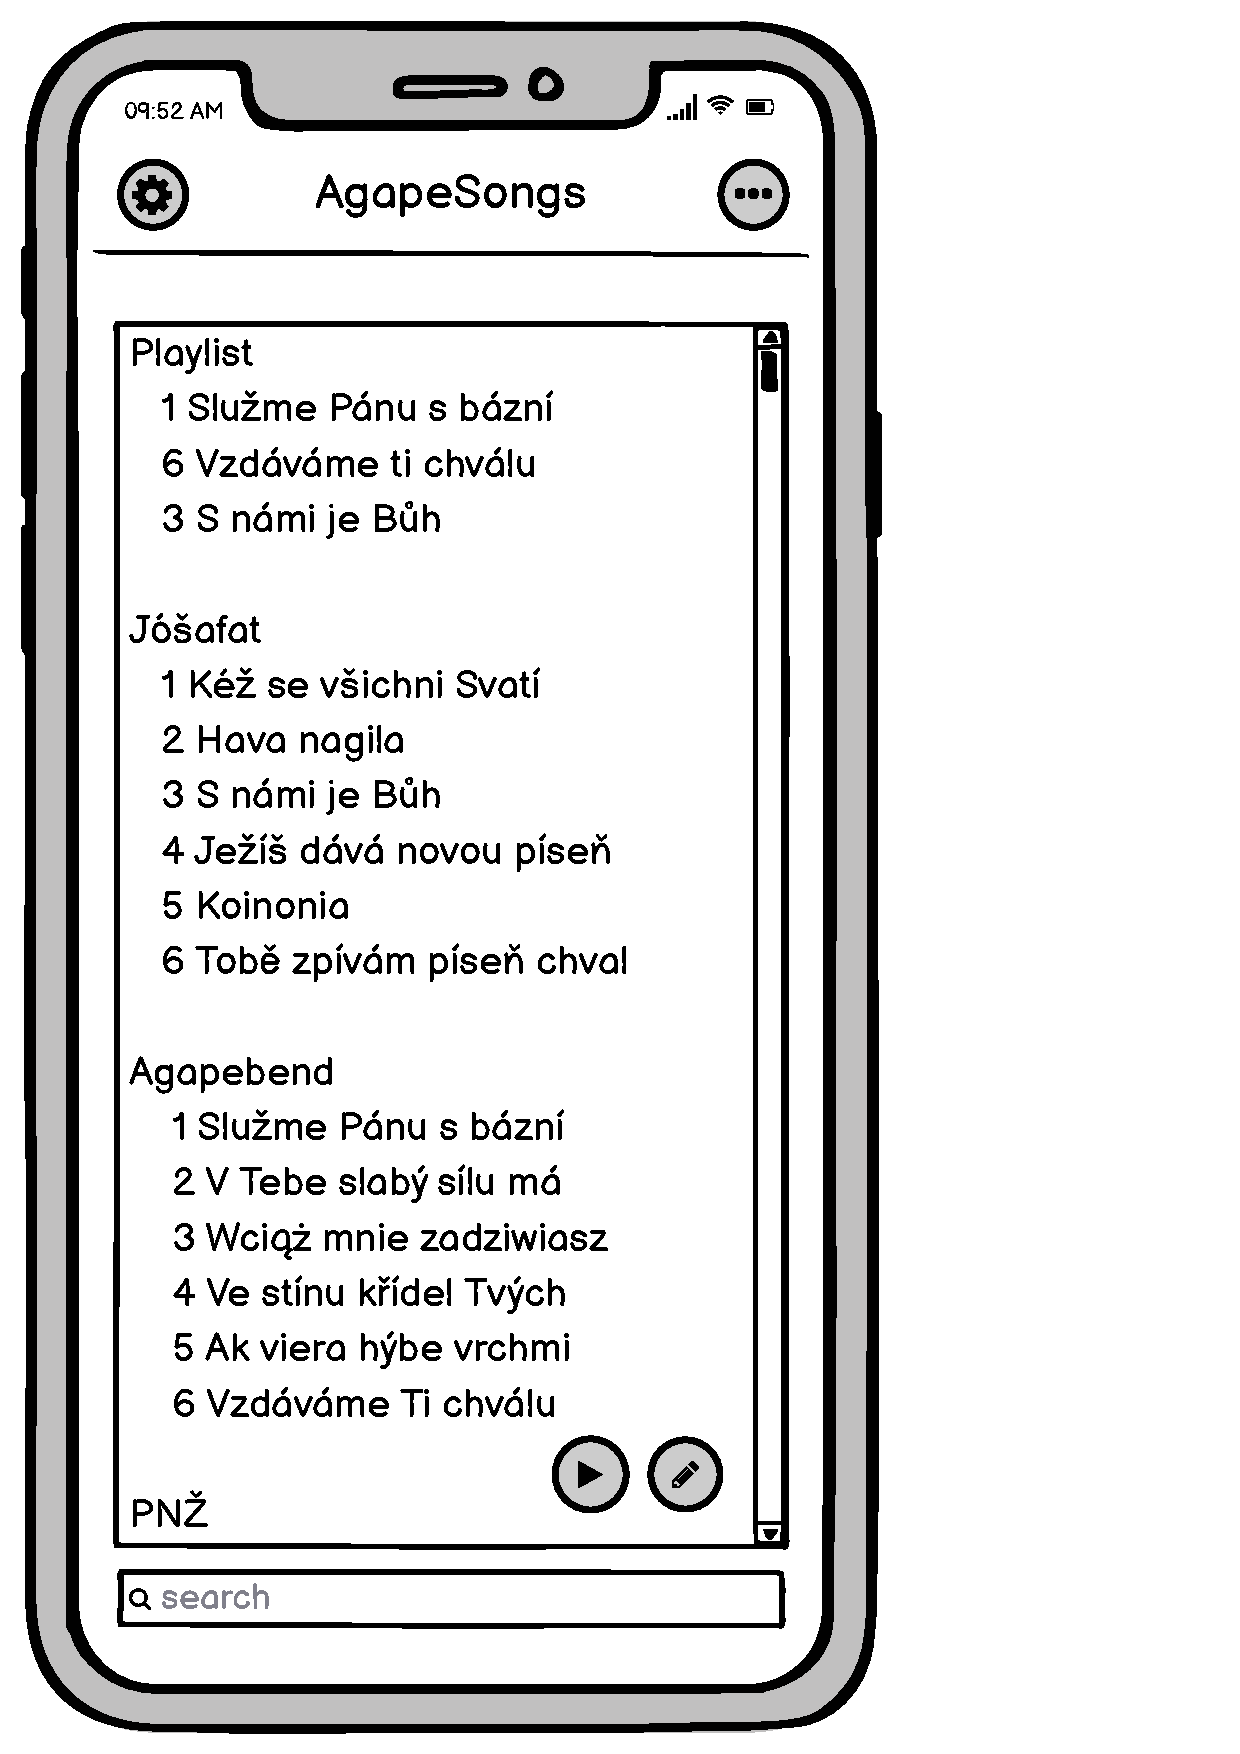
\includegraphics[width=\textwidth/3 - 2pt]{images/3-navrh/3-6-seznam-zpevniku.pdf}
    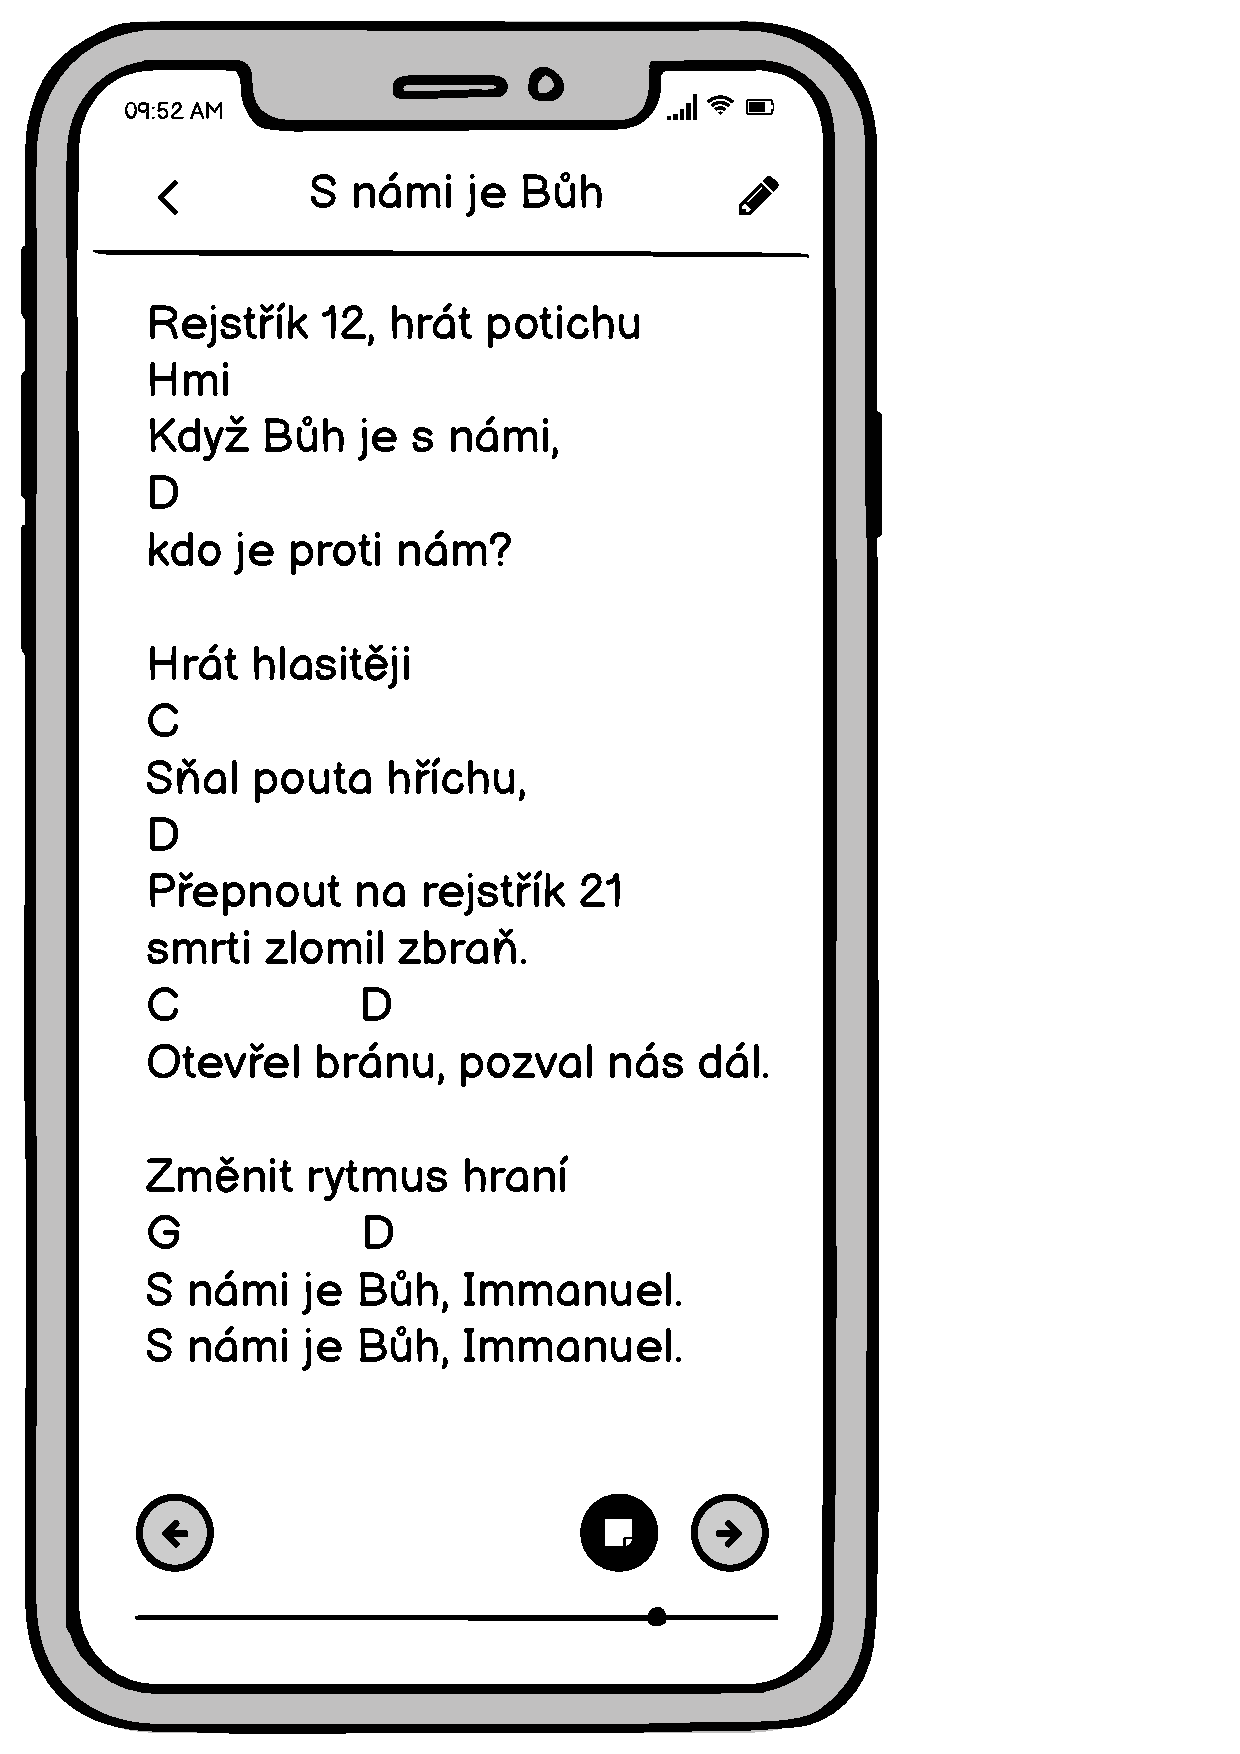
\includegraphics[width=\textwidth/3 - 2pt]{images/3-navrh/3-6-detail-pisne-clen.pdf}
    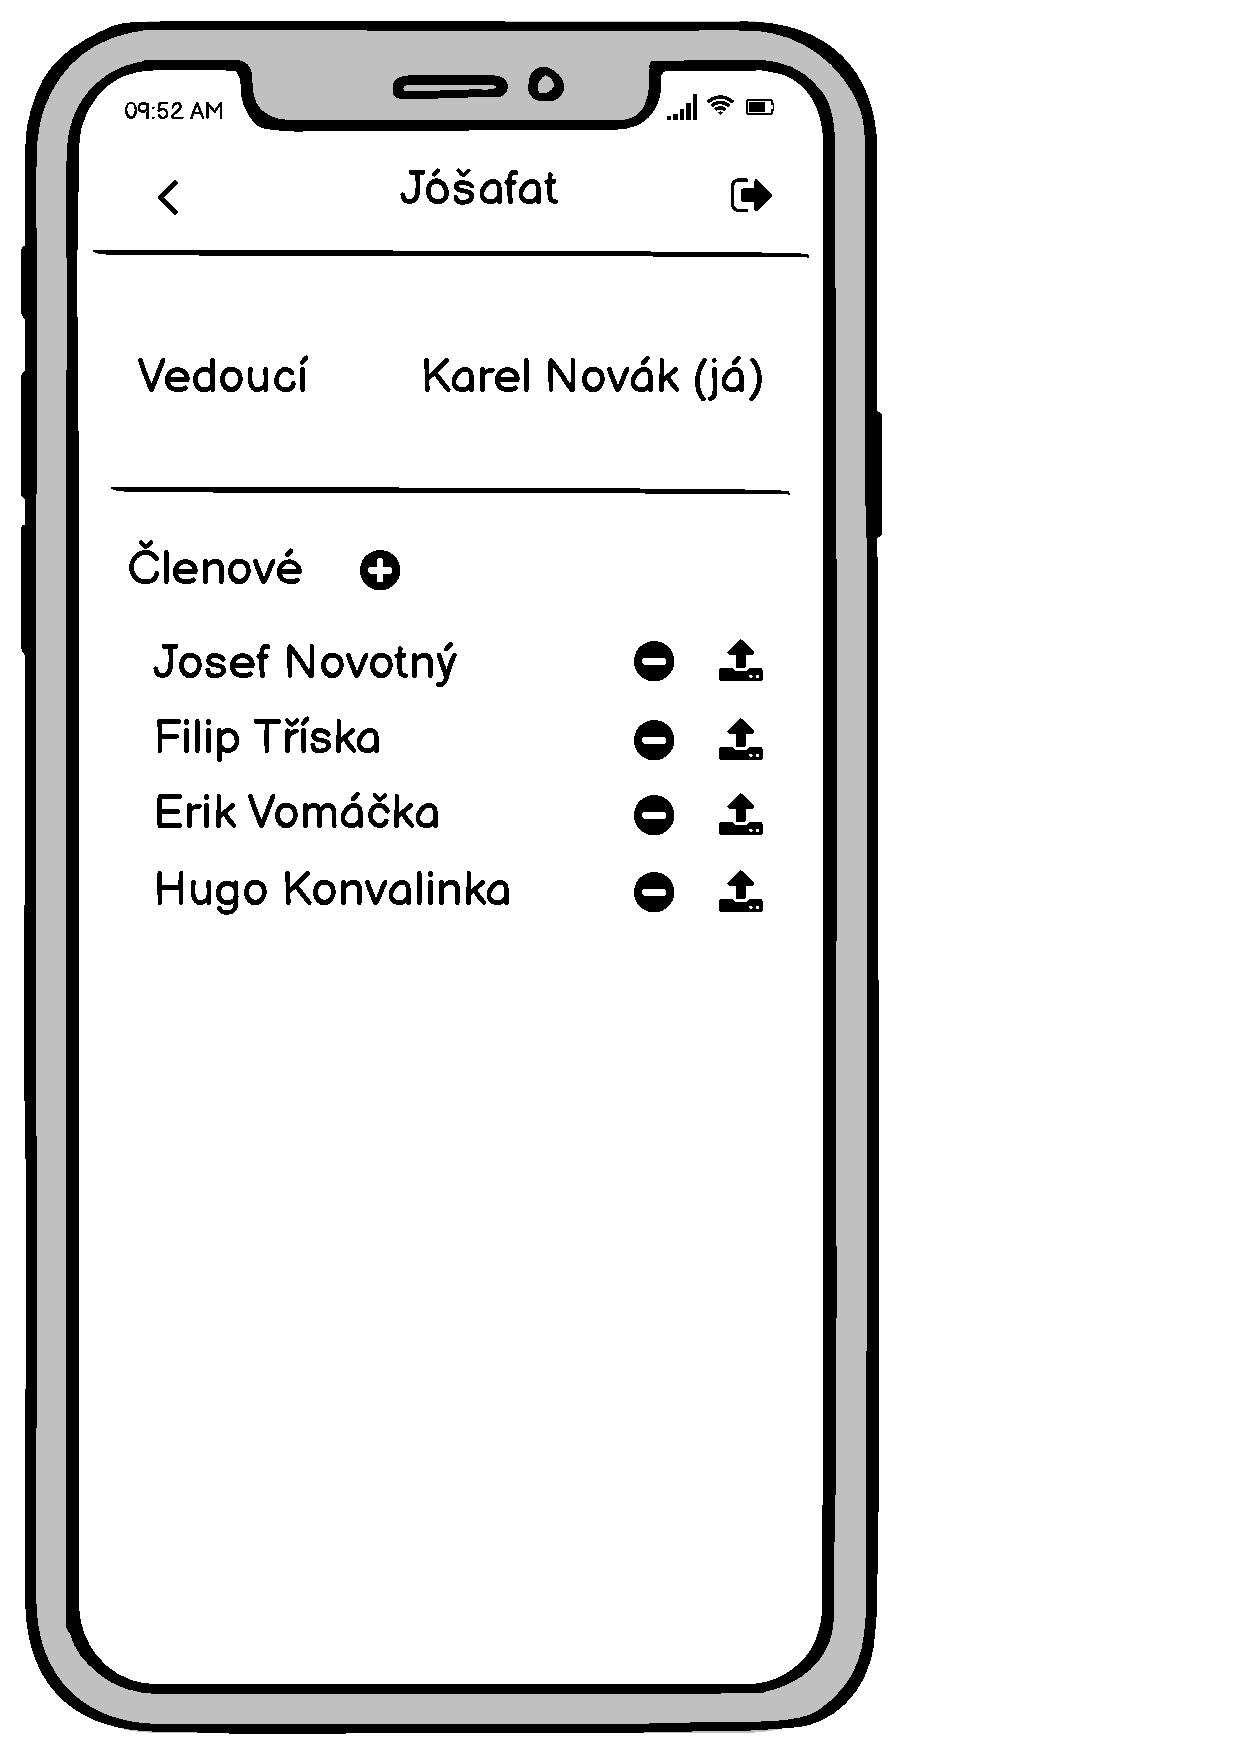
\includegraphics[width=\textwidth/3 - 2pt]{images/3-navrh/3-6-detail-kapely-vedouci.pdf}
    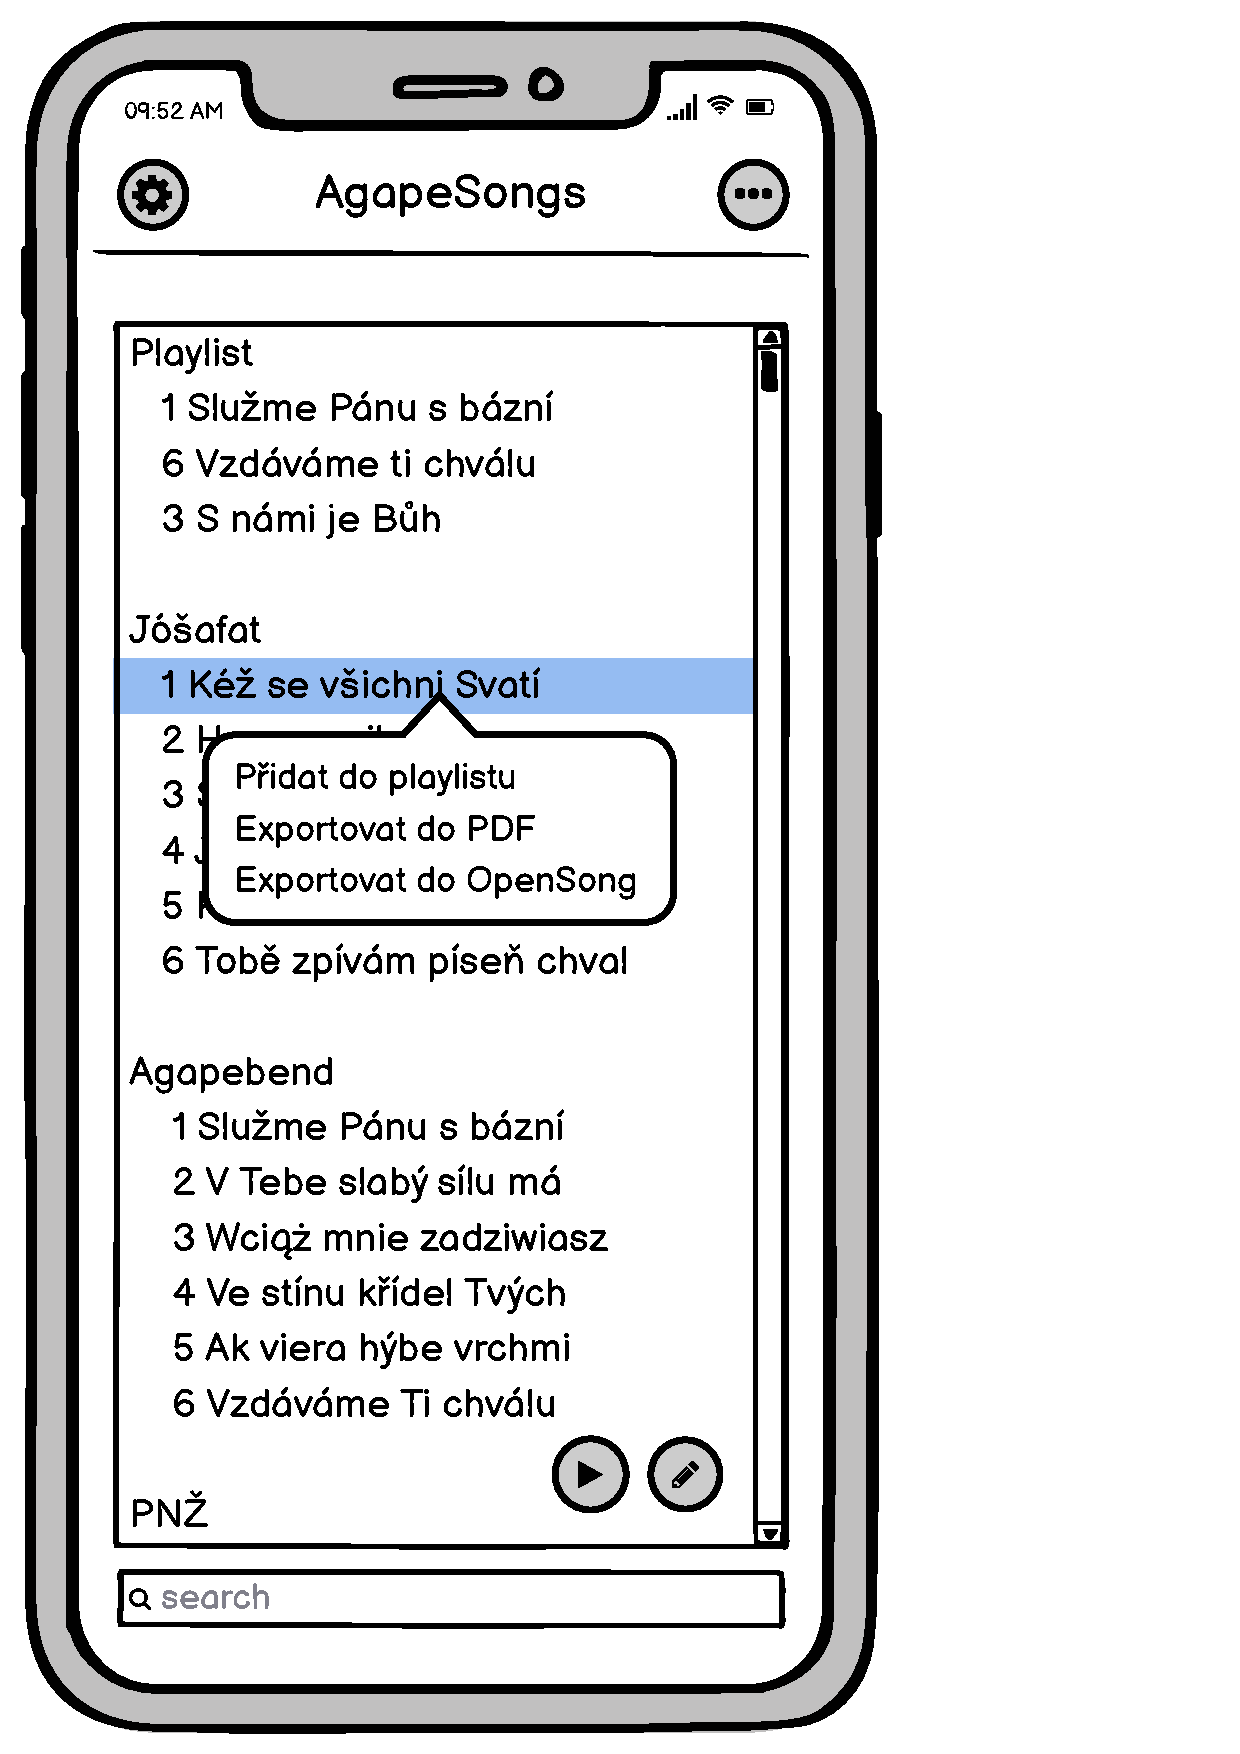
\includegraphics[width=\textwidth/3 - 2pt]{images/3-navrh/3-6-seznam-zpevniku-kontextove-menu.pdf}
    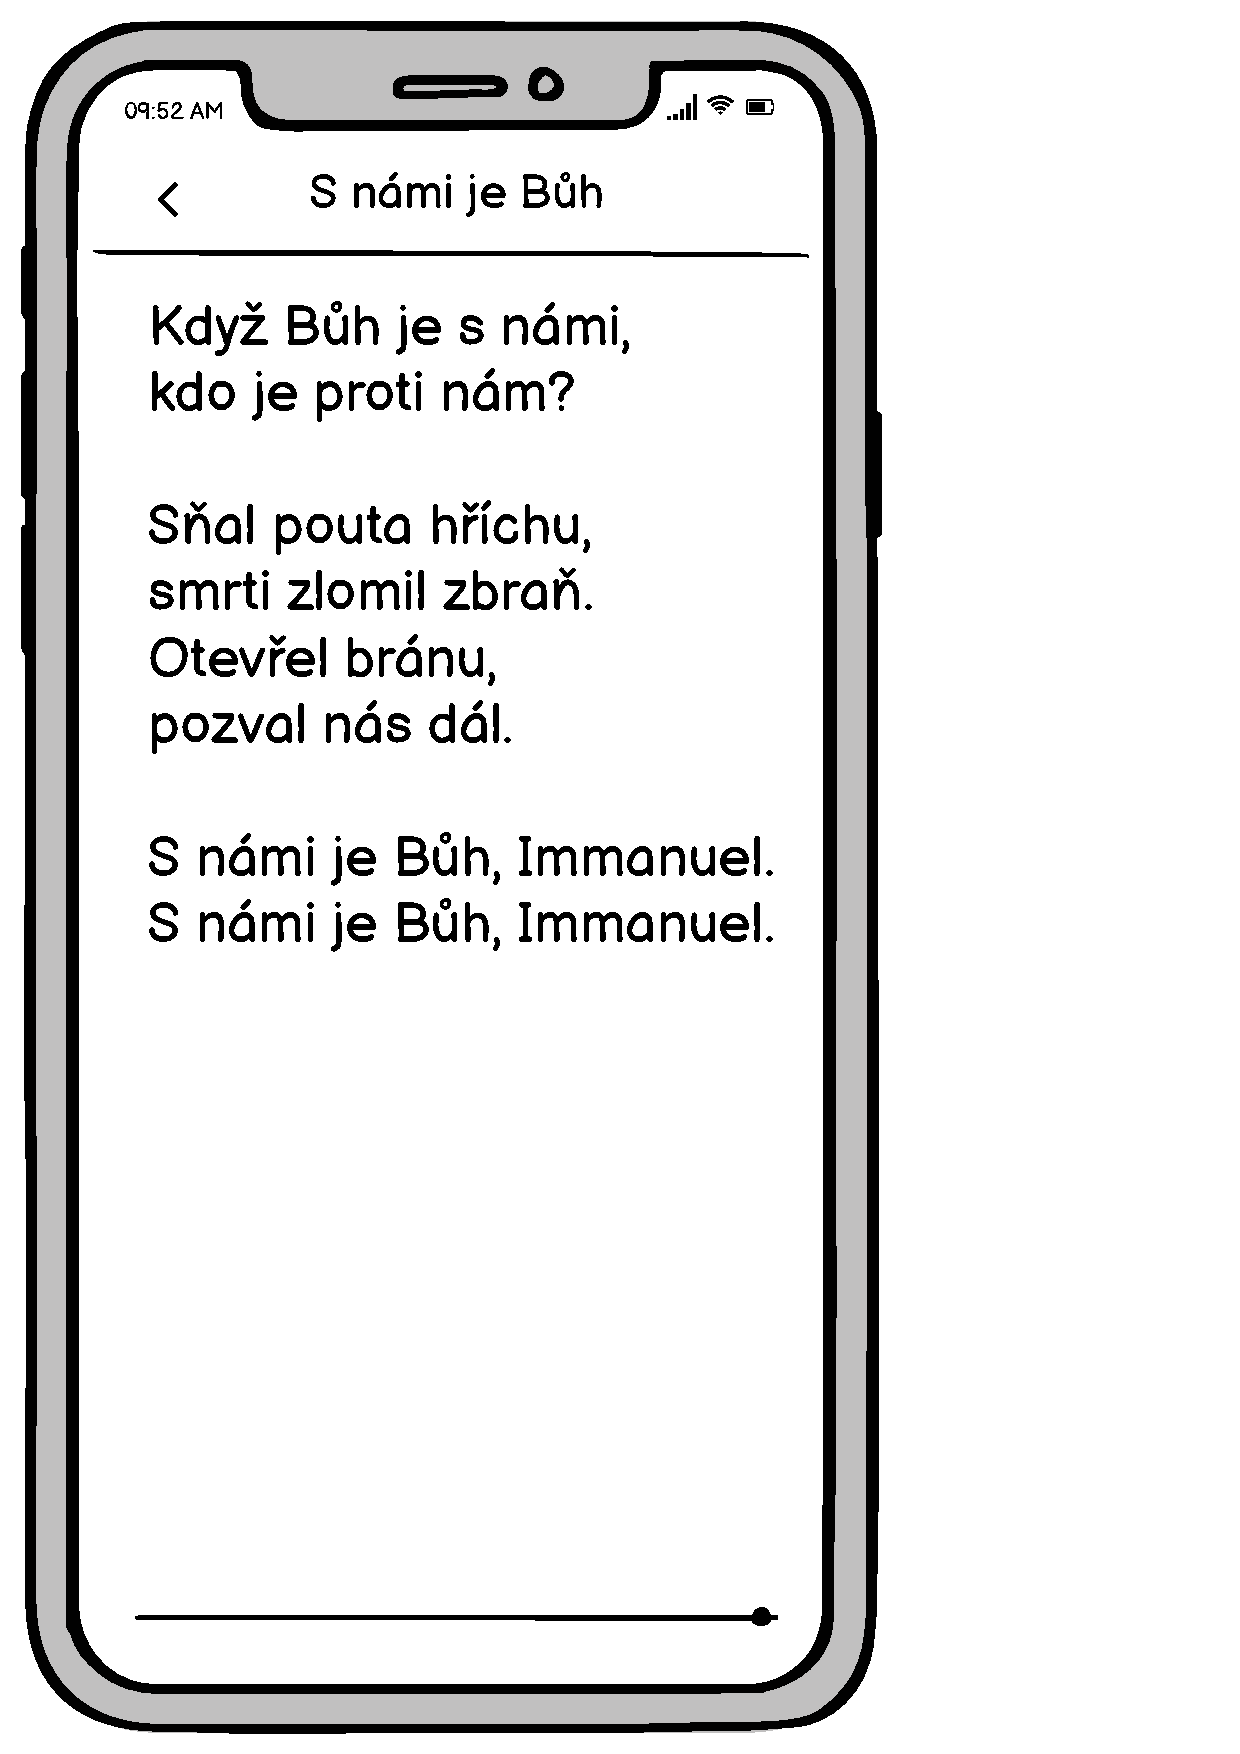
\includegraphics[width=\textwidth/3 - 2pt]{images/3-navrh/3-6-detail-pisne-host.pdf}
    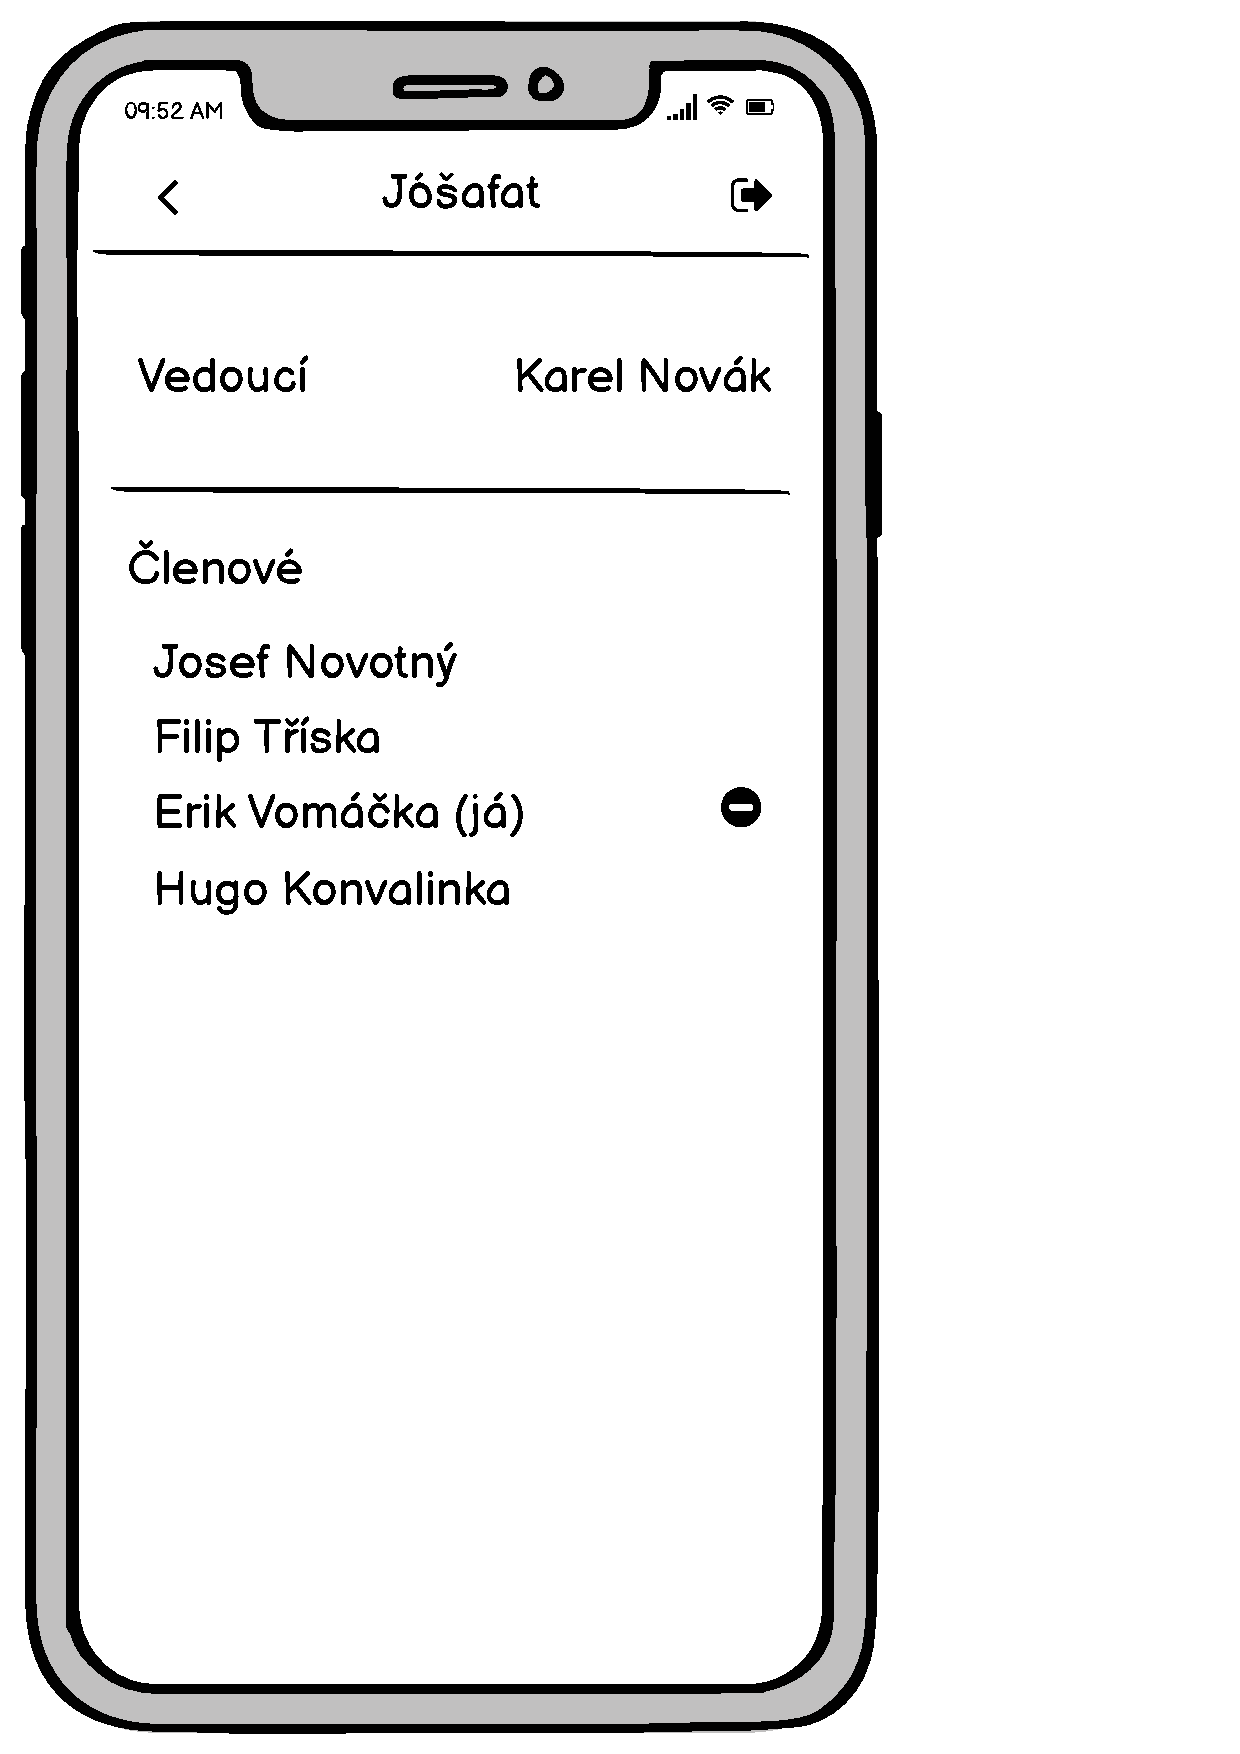
\includegraphics[width=\textwidth/3 - 2pt]{images/3-navrh/3-6-detail-kapely-clen.pdf}
    \caption[Prototyp uživatelského rozhraní -- Seznam písní, Detail písně a Detail kapely]{Prototyp uživatelského rozhraní -- Seznam písní a zpěvníků (dole s kontextovou nabídkou), Detail písně (nahoře pohled hudebníka, dole pohled zpěváka) a Detail kapely (nahoře pohled vedoucího, dole pohled člena kapely)}
\end{figure}

\subsection{Dialogy}

V aplikaci používám tři typy dialogů:

\begin{itemize}
    \item \textbf{Popover} -- dialog, který se zobrazí ve formě bubliny na tlačítku, typicky v navigační liště. V~aplikaci tento dialog používám pro filtr písní, nastavení písně a nastavení aplikace.
    \item \textbf{Sheet} -- dialog, který se zobrazí jako nová obrazovka, který lze zavřít potáhnutím dolů. Tento dialog používám pro přidávání a úpravy písní, zpěvníků a členů kapely.
    \item \textbf{Alert} -- dialog zobrazený na obrazovce se ztmavením předchozí obrazovky se dvěma možnost\-mi -- Ano, Ne. Je vhodný především pro potvrzení, ať už potvrzení odebrání zpěvníku nebo člena kapely, stáhnutí či nahrání playlistu nebo změnu oprávnění člena kapely.
\end{itemize}

\begin{figure}
    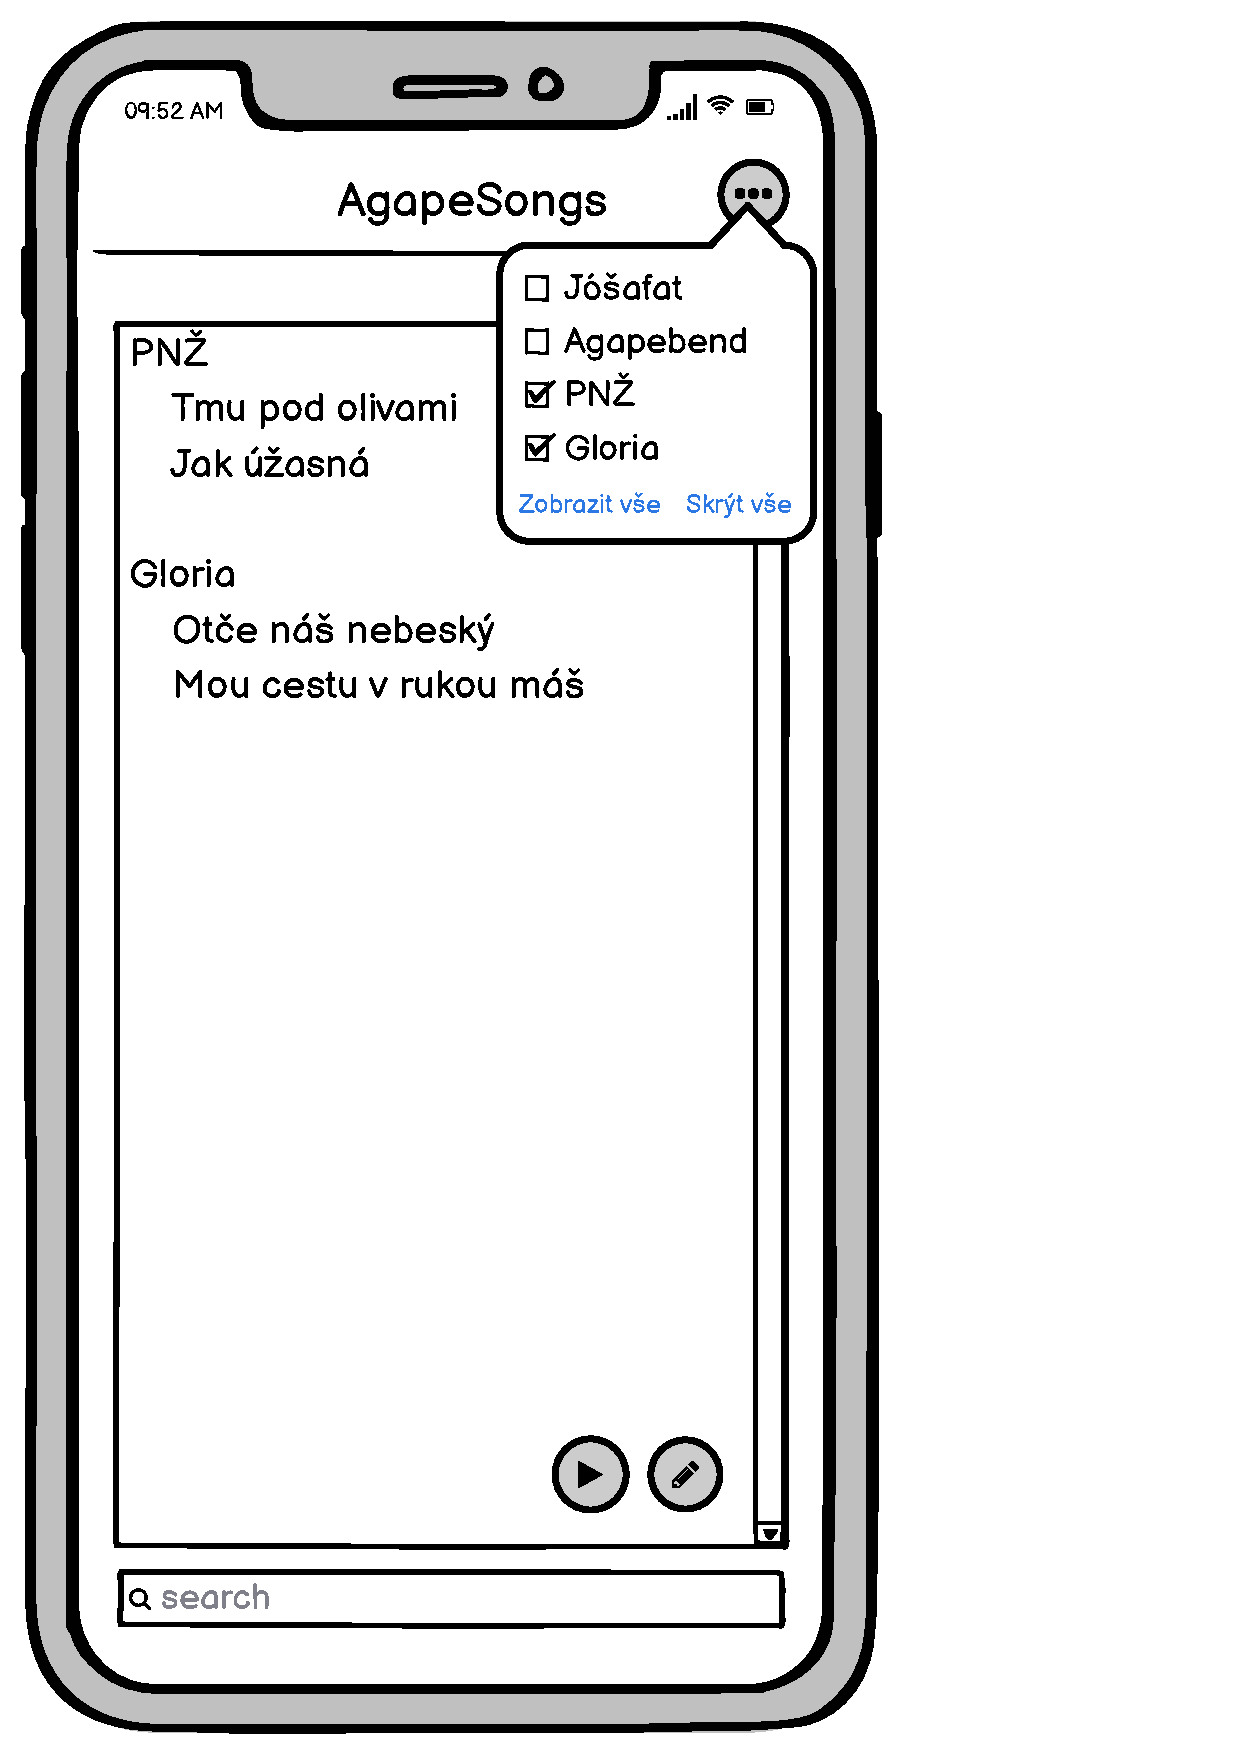
\includegraphics[width=\textwidth/3 - 2pt]{images/3-navrh/3-7-dialog-filtr-zpevniku.pdf}
    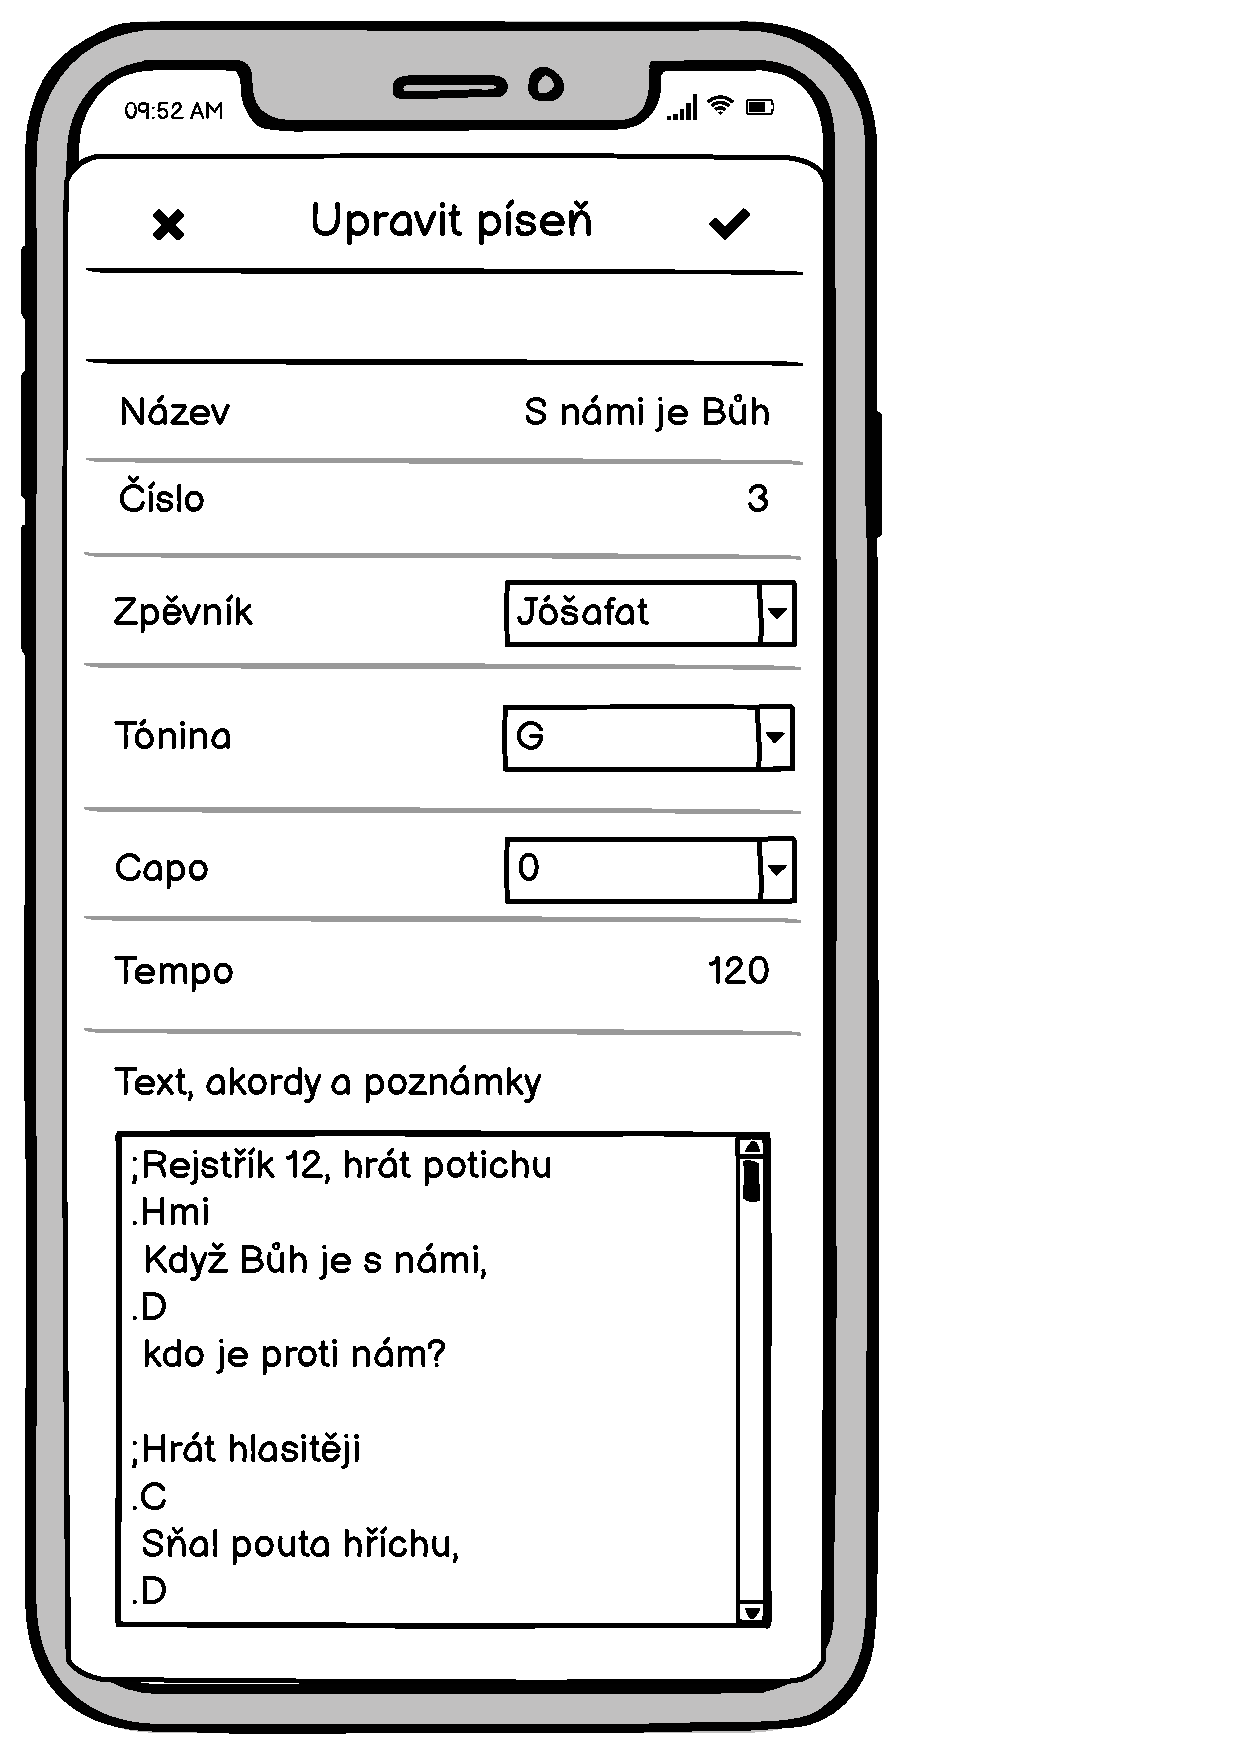
\includegraphics[width=\textwidth/3 - 2pt]{images/3-navrh/3-7-dialog-uprava.pdf}
    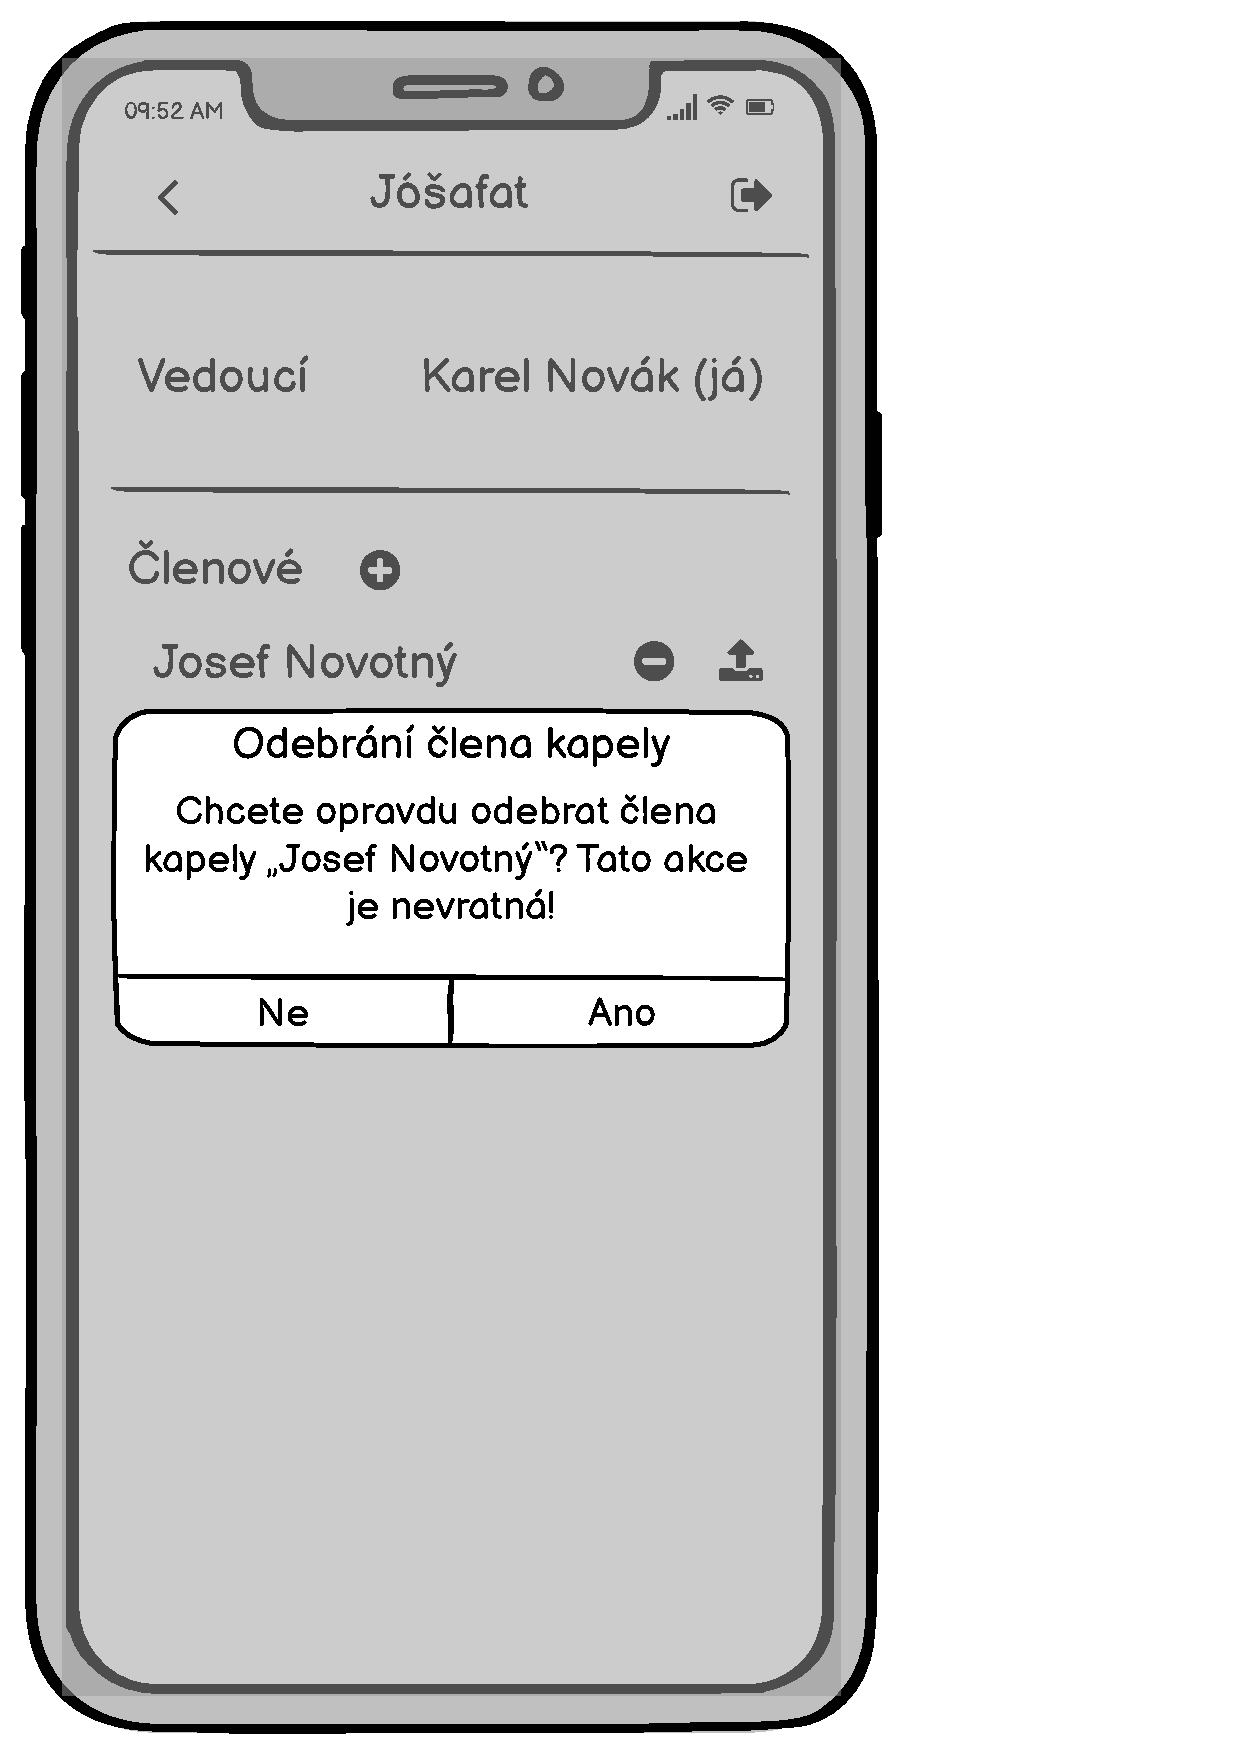
\includegraphics[width=\textwidth/3 - 2pt]{images/3-navrh/3-7-dialog-odebrani.pdf}
    \caption[Prototyp uživatelského rozhraní -- dialogy]{Prototyp uživatelského rozhraní -- Dialog pro filtr zpěvníků (popover), úpravu písně (sheet) a odebrání člena kapely (alert)}
\end{figure}
